\documentclass[a4paper,12pt,twoside]{article}


\usepackage[T1]{fontenc}
\usepackage[utf8]{inputenc}
\usepackage{lmodern}
\usepackage[french]{babel}
\usepackage{url,csquotes}
\usepackage[hidelinks,hyperfootnotes=false]{hyperref}
\usepackage[titlepage,fancysections,pagenumber,oneside]{polytechnique}
\usepackage{textcomp}
\usepackage{microtype}
\usepackage{booktabs}
\usepackage{graphicx}
\usepackage{amsmath}
\usepackage{cleveref}
\usepackage{float}
\usepackage{caption}
\graphicspath{{figures/}}
% allow common Unicode in math
\DeclareUnicodeCharacter{03BC}{\ensuremath{\mu}}
\DeclareUnicodeCharacter{207B}{\ensuremath{^-}}
\DeclareUnicodeCharacter{207A}{\ensuremath{^+}}
\DeclareUnicodeCharacter{2212}{-}
\DeclareUnicodeCharacter{2192}{\ensuremath{\to}}
\DeclareUnicodeCharacter{03B4}{\ensuremath{\delta}}
\DeclareUnicodeCharacter{1D49}{\ensuremath{\mathscr{L}}}
\DeclareUnicodeCharacter{2074}{\ensuremath{^4}}
\DeclareUnicodeCharacter{03C0}{\ensuremath{\pi}}
\DeclareUnicodeCharacter{03BD}{\ensuremath{\nu}}

% Ajout d'un environnement pour les remarques importantes
\usepackage{tcolorbox}
\newtcolorbox{remarque}{colback=gray!10!white, colframe=gray!80!black, boxrule=0.5pt, arc=2pt, left=2pt, right=2pt, top=2pt, bottom=2pt}

% Pour aérer les paragraphes
\setlength{\parskip}{0.7em}
\setlength{\parindent}{0pt}

\title{RAPPORT MODAL :\\ DÉTECTION DES MUONS}
\author{Arpad Schaeffer, Malo Tamalet}
\date{18 avril 2025}

\begin{document}

\maketitle

\tableofcontents
\listoffigures
\newpage

\section{Présentation et objectifs}
\subsection{Les Muons}
Les muons cosmiques sont des particules élémentaires de la famille des leptons, analogues à l’électron mais environ 207 fois plus massifs (masse $m_\mu \approx 105{,}7\ \mathrm{MeV}/c^2$) et dotés d’une charge électrique de $-e$ (muon négatif $\mu^-$) ou $+e$ (antimuon $\mu^+$) \cite{wikimuon,knoll2010}. Leur durée de vie propre est courte, de l’ordre de $\tau_\mu = 2{,}2\ \mu\mathrm{s}$. 

Malgré cette brièveté, les muons cosmiques sont abondamment observés au niveau du sol grâce au mécanisme de dilatation temporelle de la relativité restreinte\,:
se déplaçant à des vitesses relativistes, leurs horloges internes \og ralentissent\fg{} dans le référentiel du laboratoire, ce qui leur permet de parcourir de grandes distances avant de se désintégrer.

En effet, produits à environ 15~km d’altitude par la décomposition de mésons~$\pi$ dans les gerbes de rayons cosmiques, la plupart des muons atteignent le sol avant de se désintégrer en un électron (ou positron) et deux neutrinos, selon la réaction : $\mu^- \to e^- + \bar{\nu}_e + \nu_\mu$.

Ils ont un flux typique d’environ $1\ \text{muon}\,\mathrm{cm^{-2}}\,\mathrm{min^{-1}}$
pour les détecteurs horizontaux. Ce flux dépend fortement de l’angle d’arrivée des muons, suivant approximativement une loi en $\cos^2\theta$ (flux maximal à la verticale, $\theta=0$) du fait de l’absorption accrue dans l’atmosphère pour les trajets inclinés.

Par ailleurs, les muons cosmiques, en tant que particules très pénétrantes, interagissent peu avec la matière sur de faibles épaisseurs : ils perdent en moyenne $\sim2\ \mathrm{GeV}$ par ionisation lors de leur traversée de toute l’atmosphère, ce qui correspond à un dépôt d’énergie d’environ $1\text{-}2\ \mathrm{MeV}\,\mathrm{g^{-1}}\,\mathrm{cm^2}$
dans la matière solide (valeur typique pour un muon minimum ionisant) – une perte modeste comparée à leur énergie totale souvent de l’ordre de plusieurs GeV en arrivant au sol (énergie moyenne $\approx4\ \mathrm{GeV}$) \cite{bethe1930}.
\newpage

\subsection{Objectifs de l’étude}

\textbf{Détection et coïncidence}~: Mettre en place un télescope à scintillateurs plastiques afin de détecter les muons cosmiques et d’isoler les véritables événements muoniques du bruit de fond (bruit électronique, radioactivité naturelle, etc.). L’objectif est de comprendre l’importance de la coïncidence temporelle entre plusieurs détecteurs pour éliminer les faux signaux et garantir que seuls les muons traversant successivement plusieurs plaques sont comptés. Cette étape permet de valider la méthode de détection et d’estimer l’efficacité du dispositif.

\textbf{Distribution angulaire}~: Mesurer le flux de muons en fonction de l’angle d’incidence $\theta$ par rapport à la verticale, et vérifier expérimentalement la loi $I(\theta)\propto\cos^2\!\theta$. Cette étude met en évidence l’anisotropie du rayonnement cosmique au sol, liée à la géométrie du montage et à l’atténuation atmosphérique accrue pour les muons venant de directions inclinées. L’objectif est de confronter les mesures au modèle théorique et de comprendre l’origine physique de cette loi angulaire.

\textbf{Dépôt d’énergie}~: Étudier le pouvoir de pénétration des muons à l’aide d’absorbeurs de plomb placés sur leur trajectoire. On cherche à observer comment l’ajout d’une épaisseur de plomb réduit le flux détecté et modifie le dépôt d’énergie dans le scintillateur. Cette expérience permet de caractériser la nature très pénétrante des muons cosmiques, de quantifier leur perte d’énergie par ionisation, et d’illustrer la distribution de Landau du dépôt d’énergie.

\textbf{Temps de vie du muon}~: Chronométrer la désintégration des muons arrêtés dans un absorbeur pour déterminer expérimentalement leur temps de vie propre $\tau_\mu$. Cette mesure met en évidence la décroissance exponentielle caractéristique des particules instables et permet de comparer la valeur obtenue à la valeur de référence du modèle standard. Elle illustre aussi la dilatation du temps relativiste vécue par les muons cosmiques en vol.

\textbf{Modernisation technique}~: Remplacer les photomultiplicateurs traditionnels par des détecteurs SiPM (Silicon Photomultiplier) et utiliser un traitement numérique par FPGA pour gagner en compacité, robustesse et rapidité. L’objectif est de montrer l’apport des technologies modernes en instrumentation, d’améliorer la portabilité du dispositif, et de faciliter l’acquisition et l’analyse des données. Cette étape ouvre la voie à des applications avancées (muographie, mesures en altitude, etc.).

\newpage

\section{Montage expérimental}

% --- ENCADRÉ DÉBUT ---

\vspace{1em}
\begin{center}
\begin{tcolorbox}[colback=blue!5!white, colframe=blue!60!black, title=Principe du montage expérimental]
Détecter les muons cosmiques en isolant les vrais événements du bruit grâce à une chaîne de détection sélective. Le montage permet d’obtenir des données fiables pour l’analyse expérimentale.
\end{tcolorbox}
\end{center}

% --- FIN ENCADRÉ DÉBUT ---

Cette expérience repose sur un système de détection à scintillateur plastique couplé à un photomultiplicateurs (PM). Pour mieux comprendre la chaîne de mesure, nous décrivons ci-dessous les éléments clés, illustrés par des schémas et photos.

\begin{figure}[H]
  \centering
  \includegraphics[width=0.9\textwidth]{Images/Montage_Scintillateurs.png}
  \caption{Photo du montage de détection}
  \label{fig:setup}
\end{figure}

\newpage

\subsection{Scintillateur plastique}

% --- ENCADRÉ DÉBUT ---

\vspace{1em}
\begin{center}
\begin{tcolorbox}[colback=blue!5!white, colframe=blue!60!black, title=Principe du scintillateur plastique]
Convertir l’énergie déposée par une particule chargée en lumière visible, permettant ainsi la détection rapide et efficace des muons cosmiques.
\end{tcolorbox}
\end{center}

% --- FIN ENCADRÉ DÉBUT ---

Les scintillateurs plastiques sont des matériaux organiques capables de convertir l'énergie déposée par une particule chargée en lumière visible (scintillation). Cette technique, parmi les plus anciennes et les plus répandues pour la détection de rayonnements ionisants, repose sur la fluorescence rapide de molécules organiques intégrées dans une matrice polymère (typiquement polystyrène ou polyvinyltoluène).

Un scintillateur plastique idéal doit :
\begin{itemize}
    \item Posséder une efficacité élevée de conversion de l'énergie déposée en lumière détectable ;
    \item Présenter une réponse linéaire (le rendement lumineux est proportionnel à l'énergie déposée sur une large gamme) ;
    \item Être transparent à sa propre émission pour maximiser la collecte de lumière ;
    \item Avoir un temps de décroissance de la luminescence très court (typiquement 1--3~ns), permettant la génération de signaux rapides ;
    \item Être de bonne qualité optique et disponible en grandes dimensions ;
    \item Avoir un indice de réfraction proche de celui du verre ($\sim$1,5) pour un couplage efficace avec les photodétecteurs.
\end{itemize}
Aucun matériau ne satisfait parfaitement tous ces critères, mais les scintillateurs plastiques constituent un compromis très avantageux pour la détection de particules chargées (électrons, muons, protons, etc.), en particulier lorsqu'une grande rapidité et une géométrie flexible sont requises.

\paragraph{Mécanisme de scintillation organique~:} L'excitation d'une molécule organique par le passage d'une particule ionisante conduit à la formation d'états électroniques excités (singlets et triplets). Après relaxation rapide vers le premier état excité singulet, la désexcitation vers l'état fondamental s'accompagne de l'émission d'un photon (fluorescence rapide). La majeure partie de la lumière utile provient de cette fluorescence prompte, dont la durée de vie est de l'ordre de quelques nanosecondes. Les processus plus lents (phosphorescence, fluorescence retardée) sont négligeables pour la détection en mode impulsionnel.

\paragraph{Caractéristiques pratiques~:} Les scintillateurs plastiques sont disponibles sous forme de plaques, barres, fibres ou formes personnalisées. Leur rendement lumineux atteint typiquement 60--70\% de celui de l'anthracène (référence), avec une émission maximale autour de 400--430~nm (bleu/violet), bien adaptée aux photomultiplicateurs et SiPM. Leur atténuation optique (distance sur laquelle l'intensité lumineuse est divisée par deux) varie de quelques dizaines à plusieurs centaines de centimètres selon la pureté et la formulation. Leur densité ($\sim$1,03~g/cm$^3$) et leur forte teneur en hydrogène les rendent également sensibles aux neutrons rapides.

\paragraph{Avantages et limites~:} Les scintillateurs plastiques sont rapides, robustes, peu coûteux et facilement usinables en grandes surfaces. Leur rendement lumineux est inférieur à celui des cristaux inorganiques (NaI, CsI), mais leur rapidité et leur flexibilité géométrique les rendent incontournables en physique des particules (détecteurs de trajectoire, calorimètres, télescopes à muons, etc.). Leur réponse est linéaire pour les électrons et muons relativistes, mais moins efficace pour les particules lourdes (protons, $\alpha$) à cause du quenching (effet de Birks).


\begin{remarque}
\textbf{Synthèse~:} Les scintillateurs plastiques offrent une détection rapide et fiable des particules chargées, avec un bon compromis entre rendement lumineux, rapidité et robustesse. Ici, le choix du scintillateur plastique est motivé par la recherche d’une excellente précision temporelle (et non énergétique), indispensable pour la détection en coïncidence des muons.
\end{remarque}

\newpage

\subsection{Photomultiplicateur (PM)}

% --- ENCADRÉ DÉBUT ---

\vspace{1em}
\begin{center}
\begin{tcolorbox}[colback=blue!5!white, colframe=blue!60!black, title=Principe du photomultiplicateur (PM)]
Amplifier les faibles signaux lumineux issus du scintillateur pour obtenir une impulsion électrique exploitable, grâce à une cascade d’électrons dans un tube sous vide.
\end{tcolorbox}
\end{center}

% --- FIN ENCADRÉ DÉBUT ---

Ce tube sous vide comporte une photocathode (effet photoélectrique) et une série de dynodes en cascade. Chaque électron initial est multiplié en une avalanche ($10^6$ à $10^8$ électrons), amplifiant le signal jusqu’à une impulsion mesurable en sortie.

\begin{figure}[H]
  \centering
  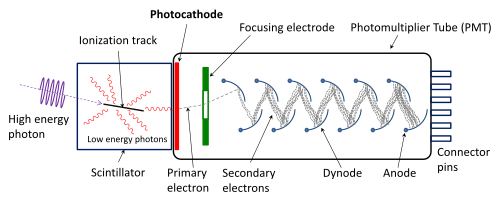
\includegraphics[width=0.7\textwidth]{Images/PhotoMultiplierTubeAndScintillator.png}
  \caption{Schéma global d’un scintillateur couplé à un photomultiplicateur}
  \label{fig:pm_scintillator}
\end{figure}

\paragraph{Principe et structure des tubes photomultiplicateurs (PM)}
Les tubes photomultiplicateurs (PM) sont essentiels pour convertir la faible lumière émise par un scintillateur en un signal électrique exploitable, avec un excellent rapport signal/bruit. Un PM est constitué d'une enveloppe sous vide, d'une photocathode photosensible et d'une chaîne de dynodes (multiplicateur d'électrons). La photocathode convertit les photons incidents en électrons (photoélectrons) par effet photoélectrique. Ces électrons sont ensuite accélérés et multipliés à chaque dynode par émission secondaire, aboutissant à un signal final amplifié de $10^6$ à $10^{10}$ électrons collectés à l'anode.

La réponse temporelle d'un PM est rapide (quelques ns), et la linéarité de l'amplification permet de conserver l'information sur l'intensité lumineuse initiale. Les PM sont disponibles dans une grande variété de tailles et de sensibilités spectrales (UV, visible, proche IR). Leur efficacité quantique (rapport entre le nombre d'électrons émis et le nombre de photons incidents) atteint typiquement 20--30\%.

\paragraph{Caractéristiques et limitations}
Les PM présentent une excellente linéarité, une faible contribution au bruit, et une grande rapidité. Cependant, ils sont sensibles aux champs magnétiques, nécessitent une alimentation haute tension (typiquement 1500 V), et doivent être protégés de la lumière ambiante pour éviter les dommages. Le bruit de fond (courant d'obscurité) provient principalement de l'émission thermique d'électrons à la photocathode, mais reste négligeable pour la détection de signaux intenses comme ceux des muons cosmiques.

\begin{remarque}
\textbf{Synthèse~:} Les PM permettent de convertir et d’amplifier efficacement la lumière en signal électrique, au prix de contraintes d’alimentation et de sensibilité à l’environnement.
\end{remarque}

\newpage

\subsection{Chaîne électronique}

% --- ENCADRÉ DÉBUT ---

\vspace{1em}
\begin{center}
\begin{tcolorbox}[colback=blue!5!white, colframe=blue!60!black, title=Principe de la chaîne électronique]
L’objectif de la chaîne électronique est d’assurer le traitement, le filtrage et la sélection des signaux issus des détecteurs afin de ne retenir que les événements pertinents. Elle permet d’optimiser la rapididité et le rapport signal/bruit, conditions essentielles pour une détection fiable et sélective des muons cosmiques.
\end{tcolorbox}
\end{center}

% --- FIN ENCADRÉ DÉBUT ---

La détection des muons nécessite une chaîne électronique rapide et fiable, composée de plusieurs instruments analogiques spécialisés. Voici les principaux modules utilisés et leur rôle dans l’expérience :

\begin{itemize}
  \item \textbf{Générateur haute tension} : Alimente les photomultiplicateurs (PM) avec une tension réglable typiquement entre 800 et 2000~V. Un réglage précis de la HT permet d’optimiser le gain du PM.
  \item \textbf{Circuit RC (filtre passe-haut)} : Placé en sortie du PM, il permet de supprimer la composante continue et d’adapter la forme du signal pour l’amplification. Le circuit RC élimine les signaux lents et ne laisse passer que les impulsions rapides des muons.
  \item \textbf{Amplificateur rapide} : Il augmente l’amplitude des signaux issus du PM pour les rendre exploitables par les modules suivants.
  \item \textbf{Discriminateur} : Ce module compare le signal amplifié à un seuil réglable (THR). Seules les impulsions dépassant ce seuil génèrent une sortie logique standard.
  \item \textbf{Retardateur} : Permet de décaler temporellement un signal logique afin d’ajuster la synchronisation entre plusieurs voies. Il est utile pour tester le taux de coïncidences fortuites ou pour compenser des différences de longueur de câble.
  \item \textbf{Module de coïncidence} : Combine les signaux logiques issus de plusieurs discriminateurs. Il délivre une impulsion uniquement si tous les signaux d’entrée arrivent dans une fenêtre temporelle variable (typiquement 10–50~ns). Cela permet de sélectionner les événements où un muon traverse plusieurs détecteurs simultanément.
  \item \textbf{Compteur} : Enregistre le nombre d’impulsions issues du module de coïncidence pendant une durée donnée. Il permet de mesurer le taux de détection.
  \item \textbf{Oscilloscope} : Permet de visualiser en temps réel les signaux analogiques à chaque étape de la chaîne (sortie PM, amplificateur, discriminateur). Il est essentiel pour ajuster les seuils et vérifier la forme des impulsions.
  \item \textbf{TAC} : Convertit le délai entre deux signaux en une tension proportionnelle. Il est utilisé pour mesurer le temps de vie des muons.
\end{itemize}

\vspace{1em}
\noindent
\textbf{Photo des instruments utilisés :}

\begin{figure}[H]
  \centering
  \includegraphics[width=0.9\textwidth]{Images/Montage_Electrique.png}
  \caption{Photo des principaux modules électroniques utilisés : générateur HT, amplificateur, discriminateur, delay, coïncidence, compteur, oscilloscope Tektronix.}
  \label{fig:photo_instruments}
\end{figure}

\begin{remarque}
\textbf{Synthèse~:} La chaîne électronique permet d’extraire efficacement les signaux utiles, d’éliminer le bruit et de garantir la fiabilité des mesures, condition essentielle pour toutes les analyses expérimentales du rapport.
\end{remarque}


\newpage

\section{Étude du signal}
\subsection{Caractérisation temporelle du signal d’un muon}

% --- ENCADRÉ DÉBUT ---

\vspace{1em}
\begin{center}
\begin{tcolorbox}[colback=blue!5!white, colframe=blue!60!black, title=Principe de l’étude du signal]
Analyser la forme, l’amplitude et la dépendance du signal détecté pour optimiser les réglages et garantir la qualité des mesures.
\end{tcolorbox}
\end{center}

% --- FIN ENCADRÉ DÉBUT ---

L’étude du signal issu de la détection d’un muon cosmique à l’aide d’un scintillateur plastique permet d’accéder à des informations précieuses sur la dynamique de la chaîne d’acquisition. Le signal typique, mesuré à l’oscilloscope, présente une décroissance exponentielle caractéristique, liée à la désexcitation des molécules du scintillateur, ainsi qu’une remontée associée à la réponse de l’électronique (constante de temps RC).

\begin{figure}[H]
    \centering
    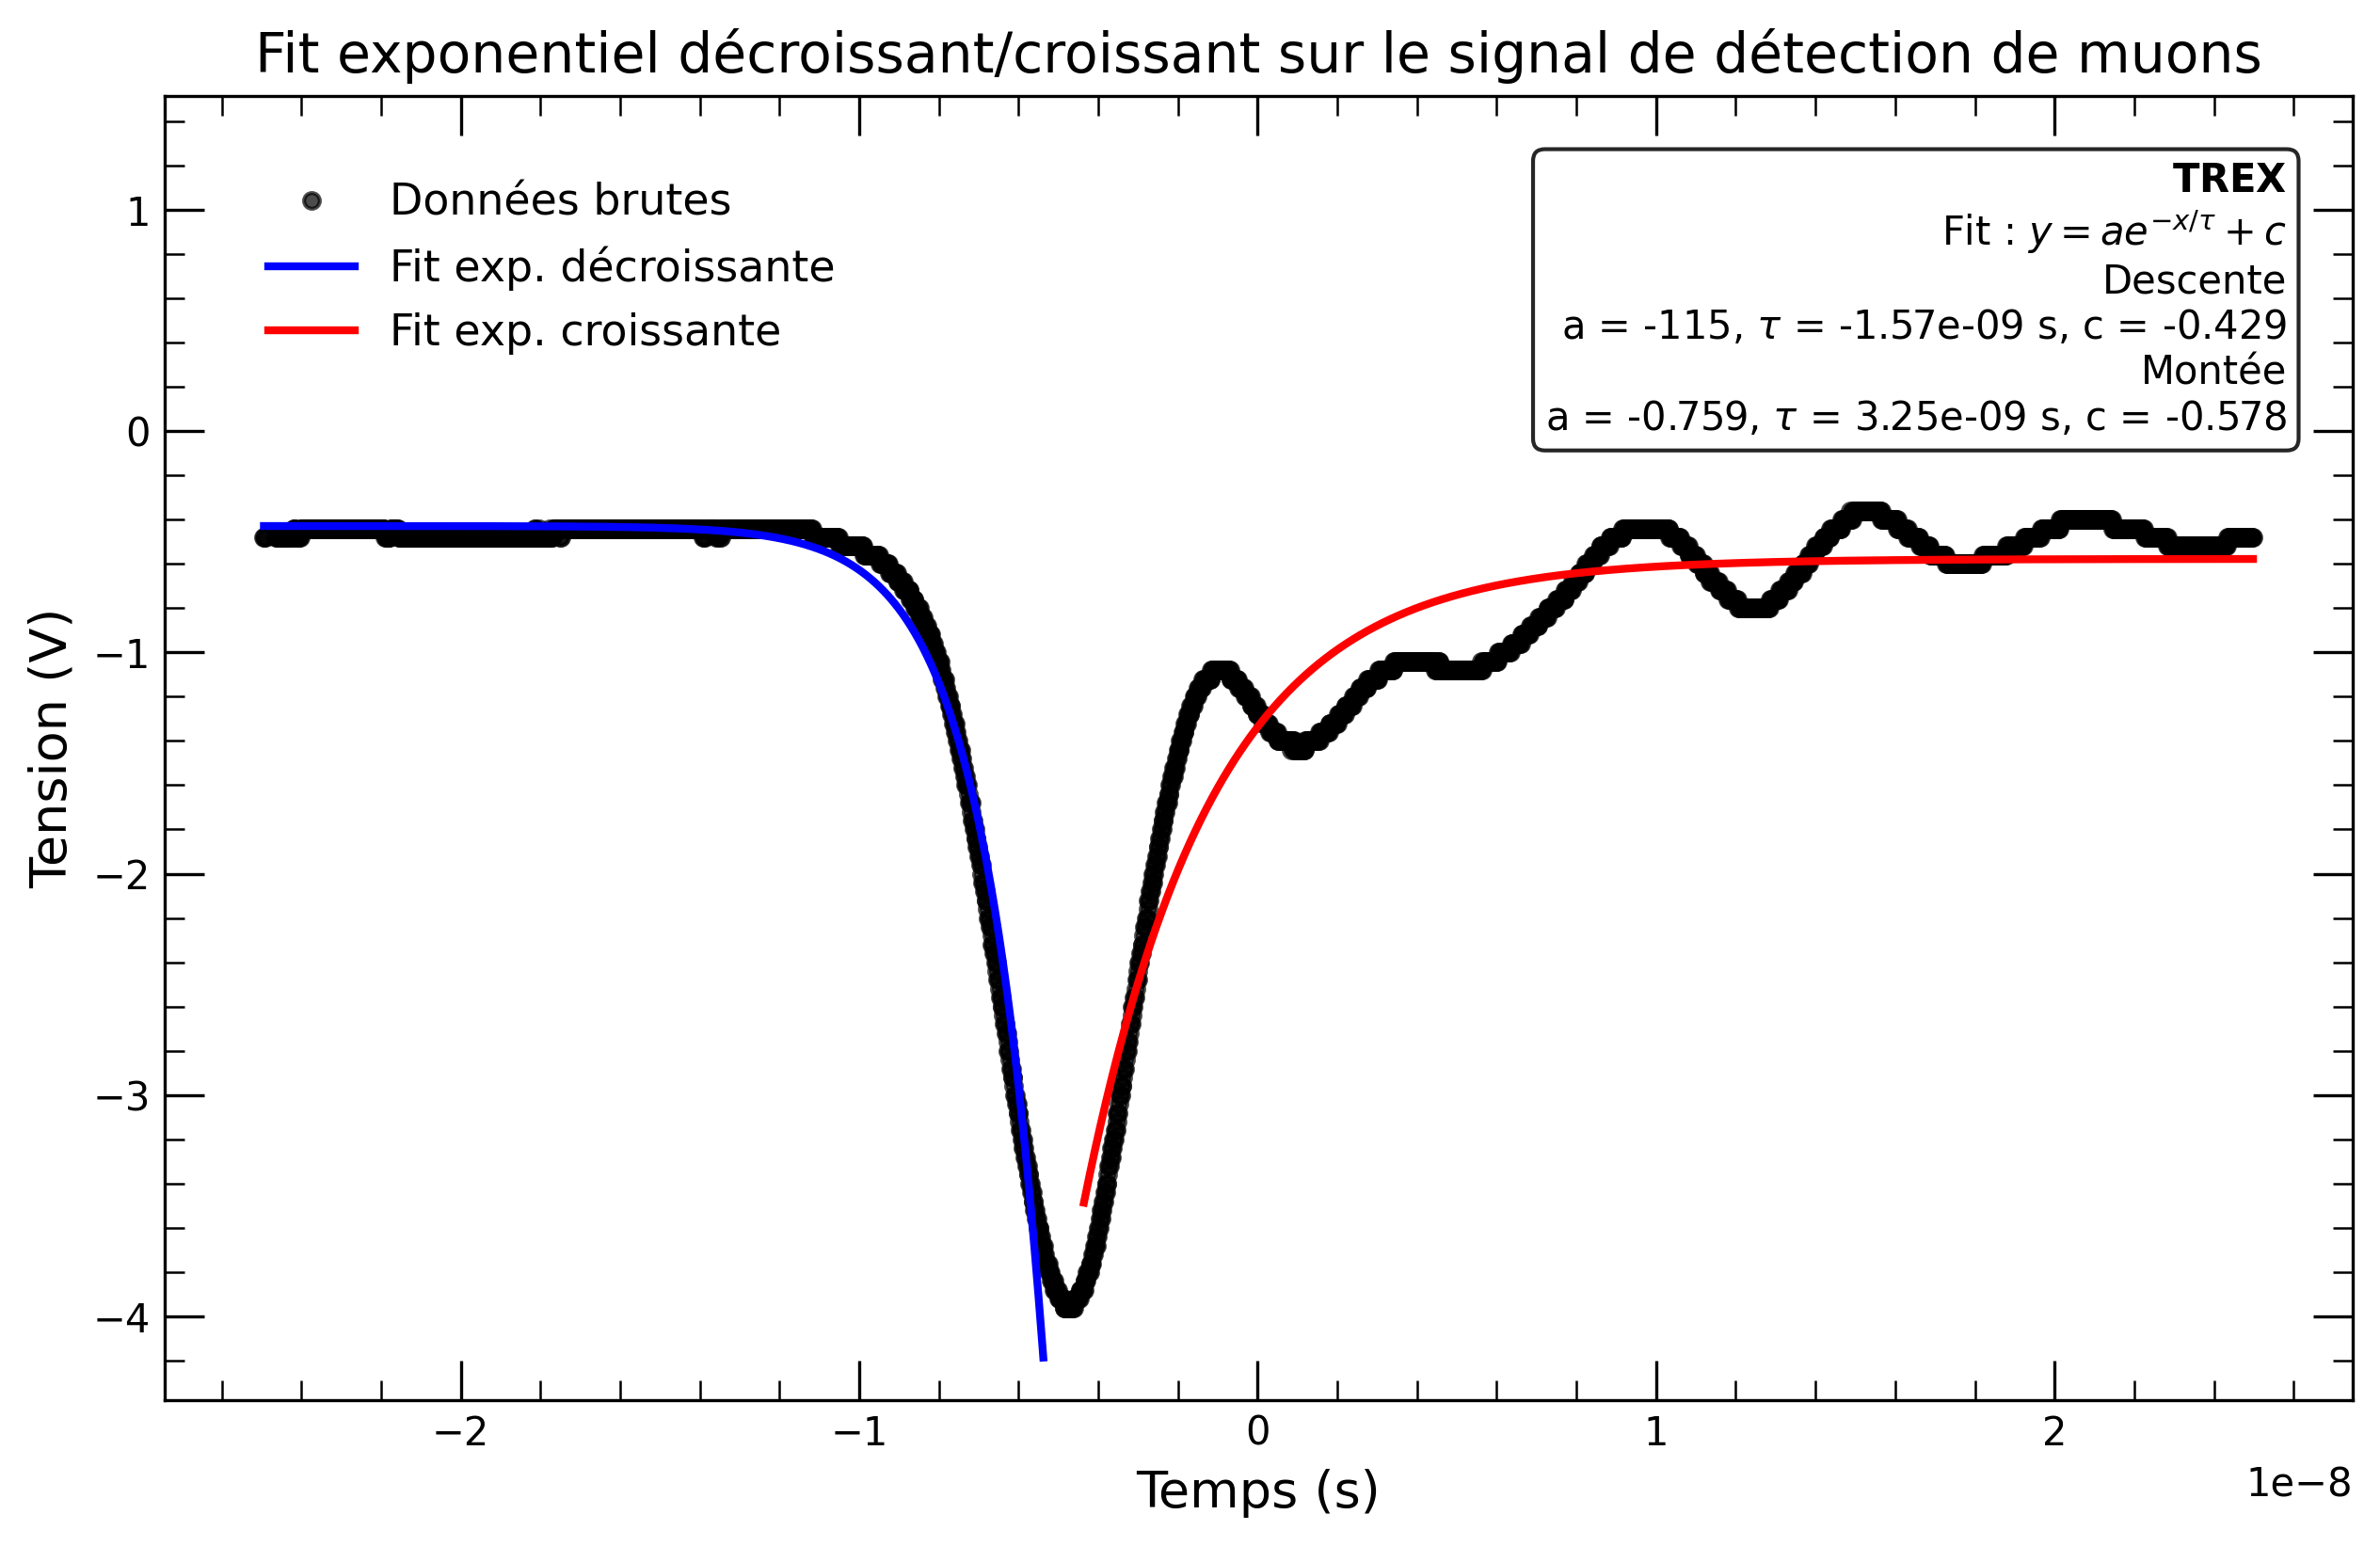
\includegraphics[width=0.9\textwidth]{Images/Desexitation_Scintillateur_2.png}
    \caption{Exemple de signal mesuré sur un muon cosmique, avec ajustements exponentiels sur la descente et la montée.}
    \label{fig:signal-muon}
\end{figure}

L’ajustement de deux exponentielles (descente et montée) sur les données expérimentales permet d’extraire deux constantes de temps :
\begin{itemize}
    \item $\tau_{\text{scint}}$ : constante de décroissance du scintillateur plastique (processus de désexcitation)
    \item $\tau_{RC}$ : constante de temps de la chaîne électronique (filtrage RC)
\end{itemize}

\begin{remarque}
\textbf{Synthèse~:} L’ajustement exponentiel du signal mesuré a permis d’extraire deux constantes caractéristiques~: $\tau_{\text{scint}} = 1{,}57$~ns (désexcitation du scintillateur) et $\tau_{RC} = 3{,}25$~ns (réponse de la chaîne électronique). La valeur obtenue pour $\tau_{\text{scint}}$ est parfaitement cohérente avec les propriétés attendues pour un scintillateur plastique, confirmant la qualité du montage et la validité de l’analyse temporelle réalisée.
\end{remarque}

\newpage

\subsection{Optimisation conjointe de la haute tension et du seuil du discriminateur}

% --- ENCADRÉ DÉBUT ---

\vspace{1em}
\begin{center}
\begin{tcolorbox}[colback=blue!5!white, colframe=blue!60!black, title=Optimisation conjointe des réglages électroniques]
Pour maximiser la détection des muons cosmiques tout en minimisant le bruit de fond, il est essentiel d’ajuster simultanément la haute tension (HT) appliquée au photomultiplicateur et le seuil du discriminateur.
\end{tcolorbox}
\end{center}

% --- FIN ENCADRÉ DÉBUT ---

\paragraph{Démarche expérimentale~:}
Pour chaque scintillateur, nous avons mesuré le nombre d’événements détectés en fonction du seuil du discriminateur, pour plusieurs valeurs de HT. Cette cartographie permet d’identifier la zone optimale où le taux de détection des muons est maximal et le bruit de fond minimal.

\begin{figure}[H]
  \centering
  

\tikzset{every picture/.style={line width=0.75pt}} %set default line width to 0.75pt        

\begin{tikzpicture}[x=0.75pt,y=0.75pt,yscale=-1,xscale=1]
%uncomment if require: \path (0,300); %set diagram left start at 0, and has height of 300

%Shape: Parallelogram [id:dp6153094668241826] 
\draw  [fill={rgb, 255:red, 155; green, 155; blue, 155 }  ,fill opacity=1 ][line width=0.75]  (234.63,54.2) -- (74.3,54.2) -- (143.01,66.72) -- (303.34,66.72) -- cycle ;
%Flowchart: Direct Access Storage [id:dp057480924744088946] 
\draw  [fill={rgb, 255:red, 74; green, 144; blue, 226 }  ,fill opacity=1 ][line width=0.75]  (327.9,63) -- (348.34,63) .. controls (351.38,63) and (353.84,59.45) .. (353.84,55.06) .. controls (353.84,50.67) and (351.38,47.12) .. (348.34,47.12) -- (327.9,47.12)(322.4,55.06) .. controls (322.4,59.45) and (324.86,63) .. (327.9,63) .. controls (330.94,63) and (333.4,59.45) .. (333.4,55.06) .. controls (333.4,50.67) and (330.94,47.12) .. (327.9,47.12) .. controls (324.86,47.12) and (322.4,50.67) .. (322.4,55.06) ;
%Shape: Triangle [id:dp281161219892323] 
\draw  [fill={rgb, 255:red, 155; green, 155; blue, 155 }  ,fill opacity=1 ][line width=0.75]  (328.02,55.6) -- (302.35,66.73) -- (234.63,54.2) -- cycle ;

%Shape: Parallelogram [id:dp9101804879233704] 
\draw  [fill={rgb, 255:red, 155; green, 155; blue, 155 }  ,fill opacity=1 ] (234.63,74.2) -- (74.3,74.2) -- (143.01,86.72) -- (303.34,86.72) -- cycle ;
%Flowchart: Direct Access Storage [id:dp015646766055150918] 
\draw  [fill={rgb, 255:red, 74; green, 144; blue, 226 }  ,fill opacity=1 ] (327.9,83) -- (348.34,83) .. controls (351.38,83) and (353.84,79.45) .. (353.84,75.06) .. controls (353.84,70.67) and (351.38,67.12) .. (348.34,67.12) -- (327.9,67.12)(322.4,75.06) .. controls (322.4,79.45) and (324.86,83) .. (327.9,83) .. controls (330.94,83) and (333.4,79.45) .. (333.4,75.06) .. controls (333.4,70.67) and (330.94,67.12) .. (327.9,67.12) .. controls (324.86,67.12) and (322.4,70.67) .. (322.4,75.06) ;
%Shape: Triangle [id:dp42632878589040457] 
\draw  [fill={rgb, 255:red, 155; green, 155; blue, 155 }  ,fill opacity=1 ] (328.02,75.6) -- (302.35,86.73) -- (234.63,74.2) -- cycle ;

%Shape: Parallelogram [id:dp08291359315510605] 
\draw  [fill={rgb, 255:red, 155; green, 155; blue, 155 }  ,fill opacity=1 ] (234.63,94.2) -- (74.3,94.2) -- (143.01,106.72) -- (303.34,106.72) -- cycle ;
%Flowchart: Direct Access Storage [id:dp39415762621948935] 
\draw  [fill={rgb, 255:red, 74; green, 144; blue, 226 }  ,fill opacity=1 ] (327.9,103) -- (348.34,103) .. controls (351.38,103) and (353.84,99.45) .. (353.84,95.06) .. controls (353.84,90.67) and (351.38,87.12) .. (348.34,87.12) -- (327.9,87.12)(322.4,95.06) .. controls (322.4,99.45) and (324.86,103) .. (327.9,103) .. controls (330.94,103) and (333.4,99.45) .. (333.4,95.06) .. controls (333.4,90.67) and (330.94,87.12) .. (327.9,87.12) .. controls (324.86,87.12) and (322.4,90.67) .. (322.4,95.06) ;
%Shape: Triangle [id:dp44810110314081986] 
\draw  [fill={rgb, 255:red, 155; green, 155; blue, 155 }  ,fill opacity=1 ] (328.02,95.6) -- (302.35,106.73) -- (234.63,94.2) -- cycle ;

%Curve Lines [id:da8784603980762927] 
\draw    (353.84,55.06) .. controls (393.84,25.06) and (392,102) .. (432,72) ;
%Curve Lines [id:da9313823595606255] 
\draw    (353.84,75.06) .. controls (393.84,45.06) and (392,102) .. (432,72) ;
%Curve Lines [id:da24872657353422778] 
\draw    (353.84,95.06) .. controls (393.84,65.06) and (392,102) .. (432,72) ;
%Shape: Rectangle [id:dp7955377352395961] 
\draw  [fill={rgb, 255:red, 208; green, 2; blue, 27 }  ,fill opacity=1 ] (432,48) -- (456.24,48) -- (456.24,96) -- (432,96) -- cycle ;
%Shape: Frame [id:dp790746320543737] 
\draw   (564,12) -- (634,12) -- (634,52) -- (564,52) -- cycle(628,18) -- (570,18) -- (570,46) -- (628,46) -- cycle ;
%Shape: Rectangle [id:dp8336691747772105] 
\draw   (313.2,116.11) -- (368.64,116.11) -- (368.64,121.89) -- (313.2,121.89) -- cycle ;
%Shape: Rectangle [id:dp6493800754350441] 
\draw   (313.2,121.89) -- (368.64,121.89) -- (368.64,127.68) -- (313.2,127.68) -- cycle ;
%Shape: Rectangle [id:dp7269506258160386] 
\draw   (313.2,110.32) -- (368.64,110.32) -- (368.64,116.11) -- (313.2,116.11) -- cycle ;

%Straight Lines [id:da6829845507956613] 
\draw    (340.64,102.64) -- (340.64,110.2) ;
%Straight Lines [id:da5330000370742687] 
\draw    (340.4,82.89) -- (340.49,87.27) ;
%Straight Lines [id:da5174947670175065] 
\draw    (339.78,62.58) -- (339.87,66.97) ;
%Shape: Rectangle [id:dp7820496204409214] 
\draw  [fill={rgb, 255:red, 74; green, 144; blue, 226 }  ,fill opacity=1 ] (479.76,48) -- (504,48) -- (504,96) -- (479.76,96) -- cycle ;
%Shape: Frame [id:dp44415473016363605] 
\draw   (564,80) -- (634,80) -- (634,120) -- (564,120) -- cycle(628,86) -- (570,86) -- (570,114) -- (628,114) -- cycle ;
%Curve Lines [id:da7027674246282678] 
\draw    (504,72) .. controls (544,42) and (524.71,27.29) .. (564,36) ;
%Curve Lines [id:da161234971098009] 
\draw    (504,72) .. controls (544,42) and (524,126) .. (564,96) ;
%Straight Lines [id:da2592906745330712] 
\draw    (456,60) -- (492,60) ;
\draw [shift={(492,60)}, rotate = 0] [color={rgb, 255:red, 0; green, 0; blue, 0 }  ][fill={rgb, 255:red, 0; green, 0; blue, 0 }  ][line width=0.75]      (0, 0) circle [x radius= 3.35, y radius= 3.35]   ;
%Straight Lines [id:da4896356965331372] 
\draw    (456,72) -- (492,72) ;
\draw [shift={(492,72)}, rotate = 0] [color={rgb, 255:red, 0; green, 0; blue, 0 }  ][fill={rgb, 255:red, 0; green, 0; blue, 0 }  ][line width=0.75]      (0, 0) circle [x radius= 3.35, y radius= 3.35]   ;
%Straight Lines [id:da963095590048375] 
\draw    (456,84) -- (492,84) ;
\draw [shift={(492,84)}, rotate = 0] [color={rgb, 255:red, 0; green, 0; blue, 0 }  ][fill={rgb, 255:red, 0; green, 0; blue, 0 }  ][line width=0.75]      (0, 0) circle [x radius= 3.35, y radius= 3.35]   ;

% Text Node
\draw (574,17) node [anchor=north west][inner sep=0.75pt]   [align=left] {{\tiny \textbf{Oscilloscope}}};
% Text Node
\draw (420,27) node [anchor=north west][inner sep=0.75pt]   [align=left] {{\tiny Amplificateur}};
% Text Node
\draw (328.8,27) node [anchor=north west][inner sep=0.75pt]   [align=left] {{\tiny PMTs}};
% Text Node
\draw (186.4,28.2) node [anchor=north west][inner sep=0.75pt]   [align=left] {{\tiny Scintillateurs}};
% Text Node
\draw (310,130) node [anchor=north west][inner sep=0.75pt]   [align=left] {{\tiny Haute Tension}};
% Text Node
\draw (465,110) node [anchor=north west][inner sep=0.75pt]   [align=left] {{\tiny Discriminateur}};
% Text Node
\draw (578,97) node [anchor=north west][inner sep=0.75pt]  [font=\footnotesize] [align=left] {{\fontfamily{pcr}\selectfont {\footnotesize \textcolor[rgb]{1,0,0}{000}}}};
% Text Node
\draw (607,96) node [anchor=north west][inner sep=0.75pt]  [font=\footnotesize] [align=left] {{\fontfamily{pcr}\selectfont {\tiny \textcolor[rgb]{1,0,0}{600s}}}};
% Text Node
\draw (572,81) node [anchor=north west][inner sep=0.75pt]   [align=left] {{\tiny \textbf{Compteur}}};


\end{tikzpicture}

  \caption{Schéma de la chaîne électronique utilisée pour faire varier le seuil du discriminateur.}
  \label{fig:variation_seuil}
\end{figure}

% Trois figures séparées pour chaque scintillateur

\begin{figure}[H]
    \centering
    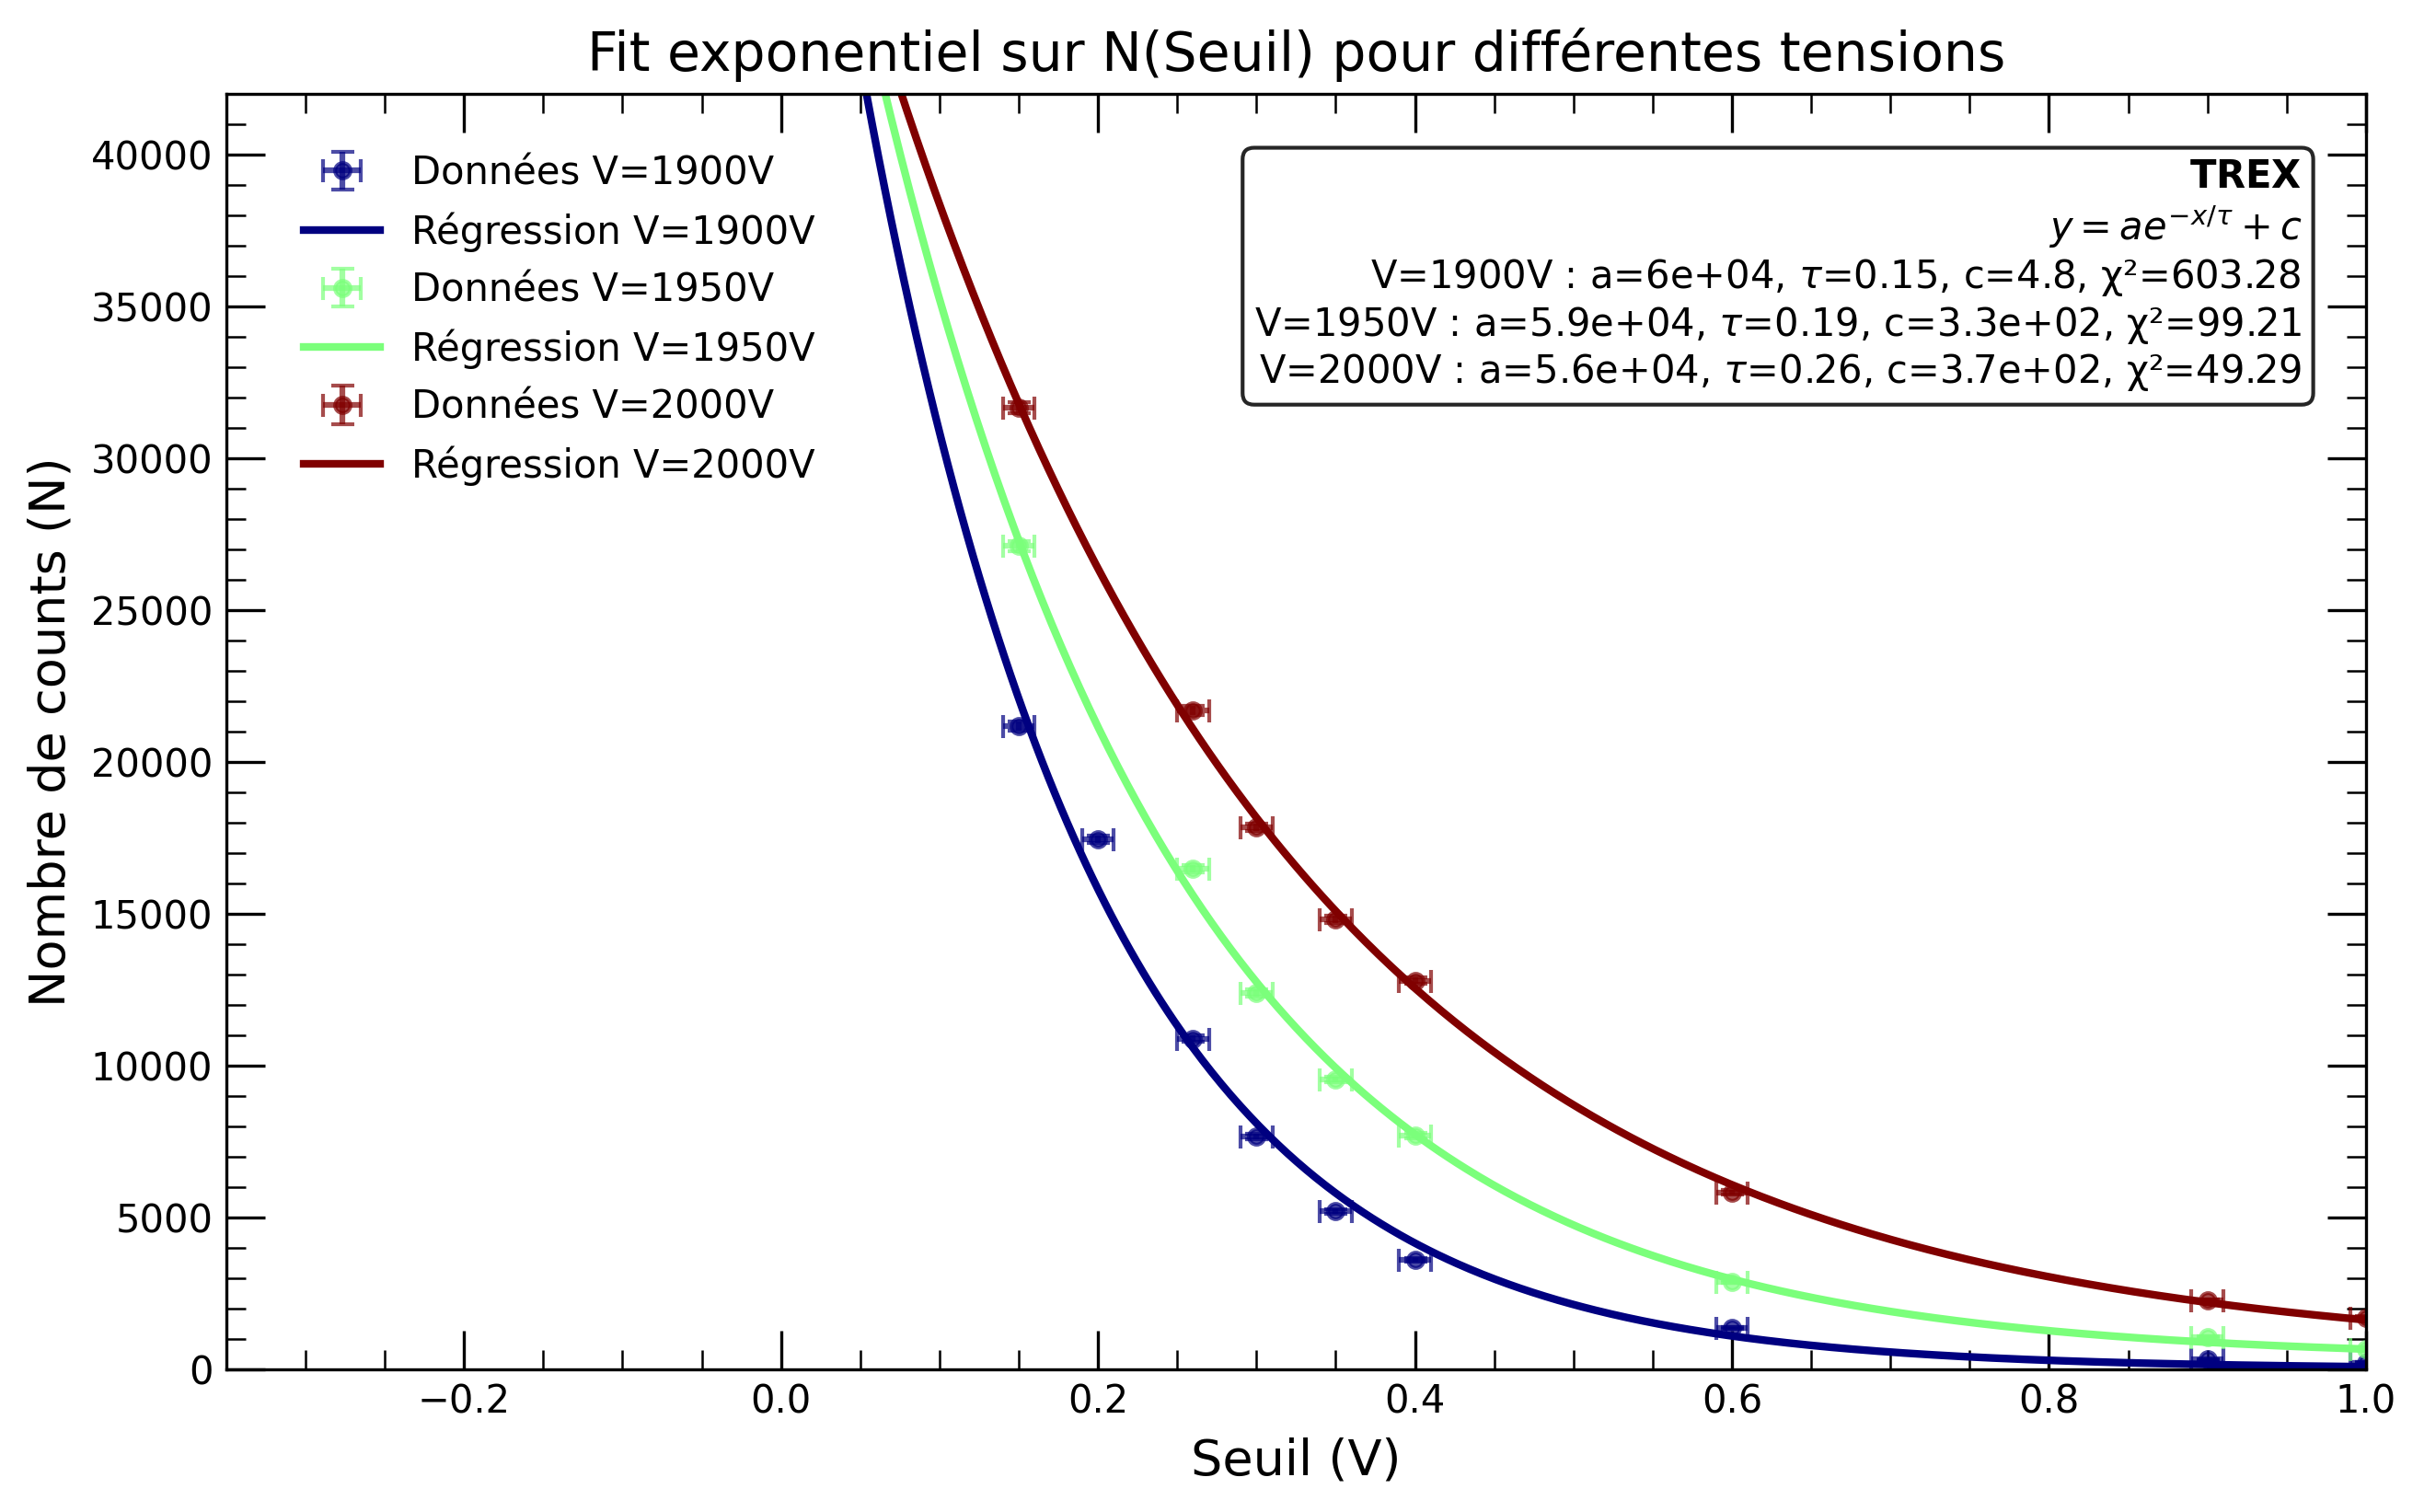
\includegraphics[width=0.9\textwidth]{Images/Threshold_Scintillateur_1.png}
    \caption{Nombre d’événements détectés en fonction du seuil pour différentes HT (Scintillateur 1).}
    \label{fig:optimisation_scint1}
\end{figure}

\begin{figure}[H]
    \centering
    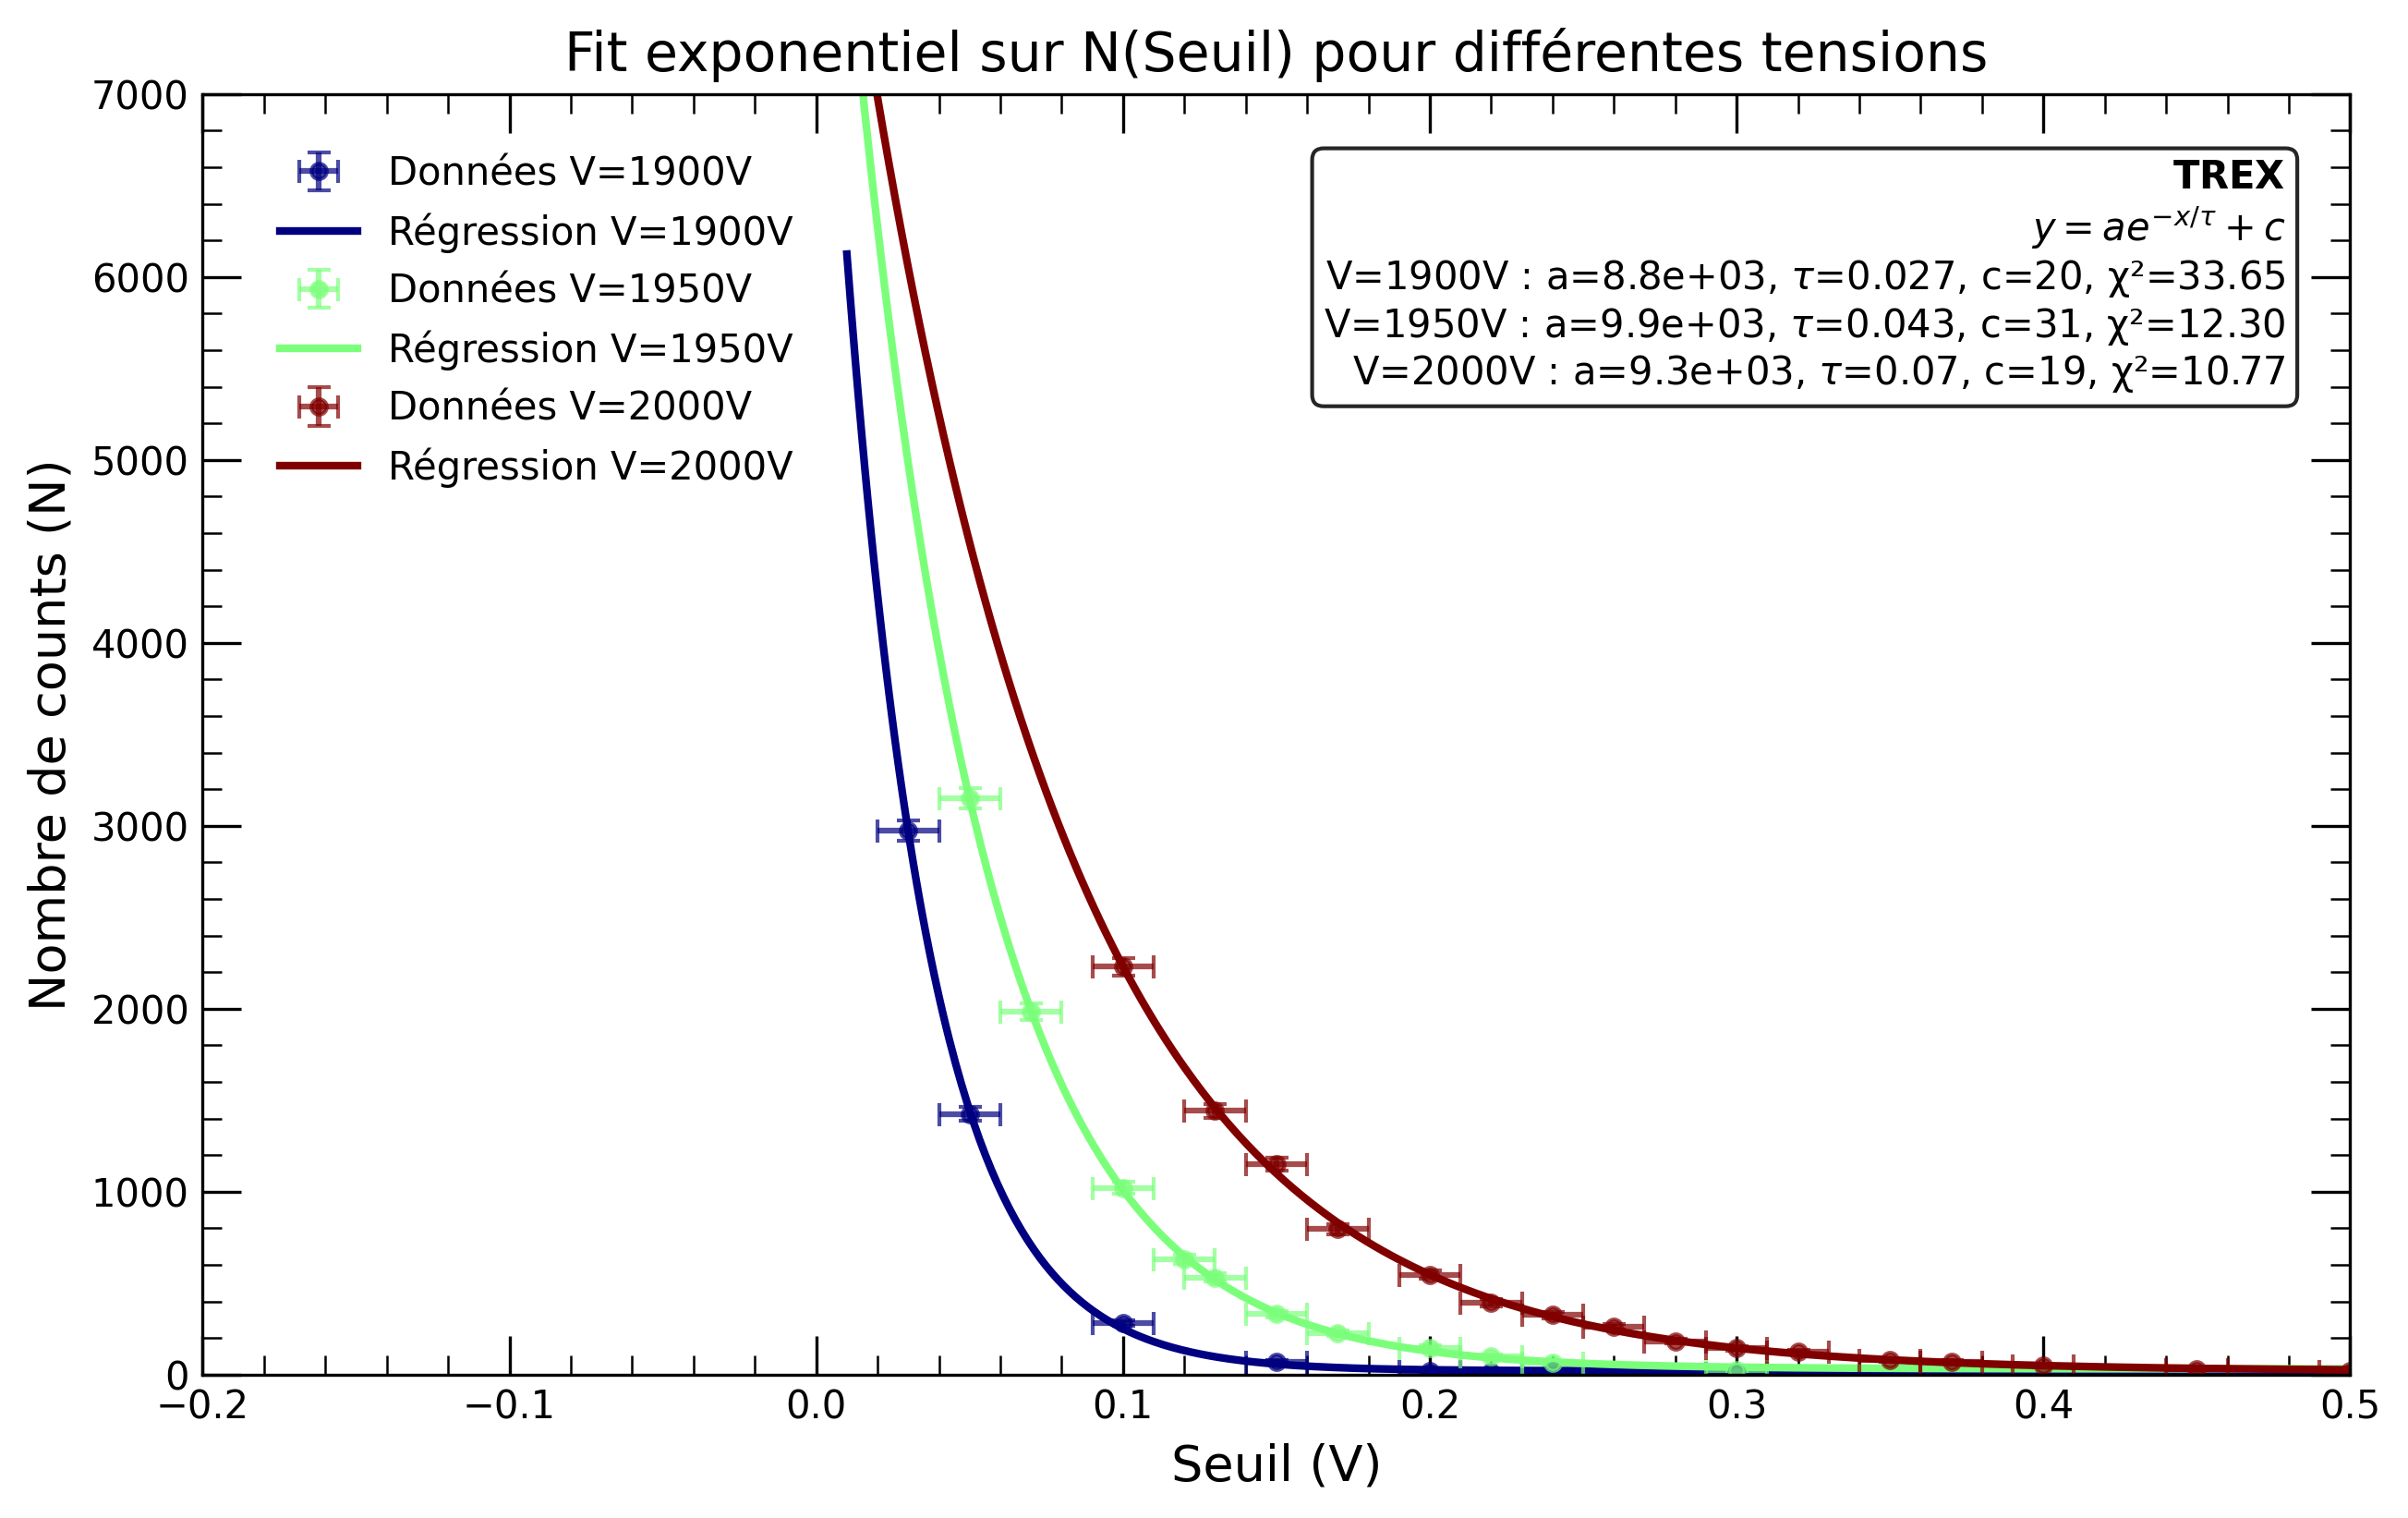
\includegraphics[width=0.9\textwidth]{Images/Threshold_Scintillateur_2.png}
    \caption{Nombre d’événements détectés en fonction du seuil pour différentes HT (Scintillateur 2).}
    \label{fig:optimisation_scint2}
\end{figure}

\begin{figure}[H]
    \centering
    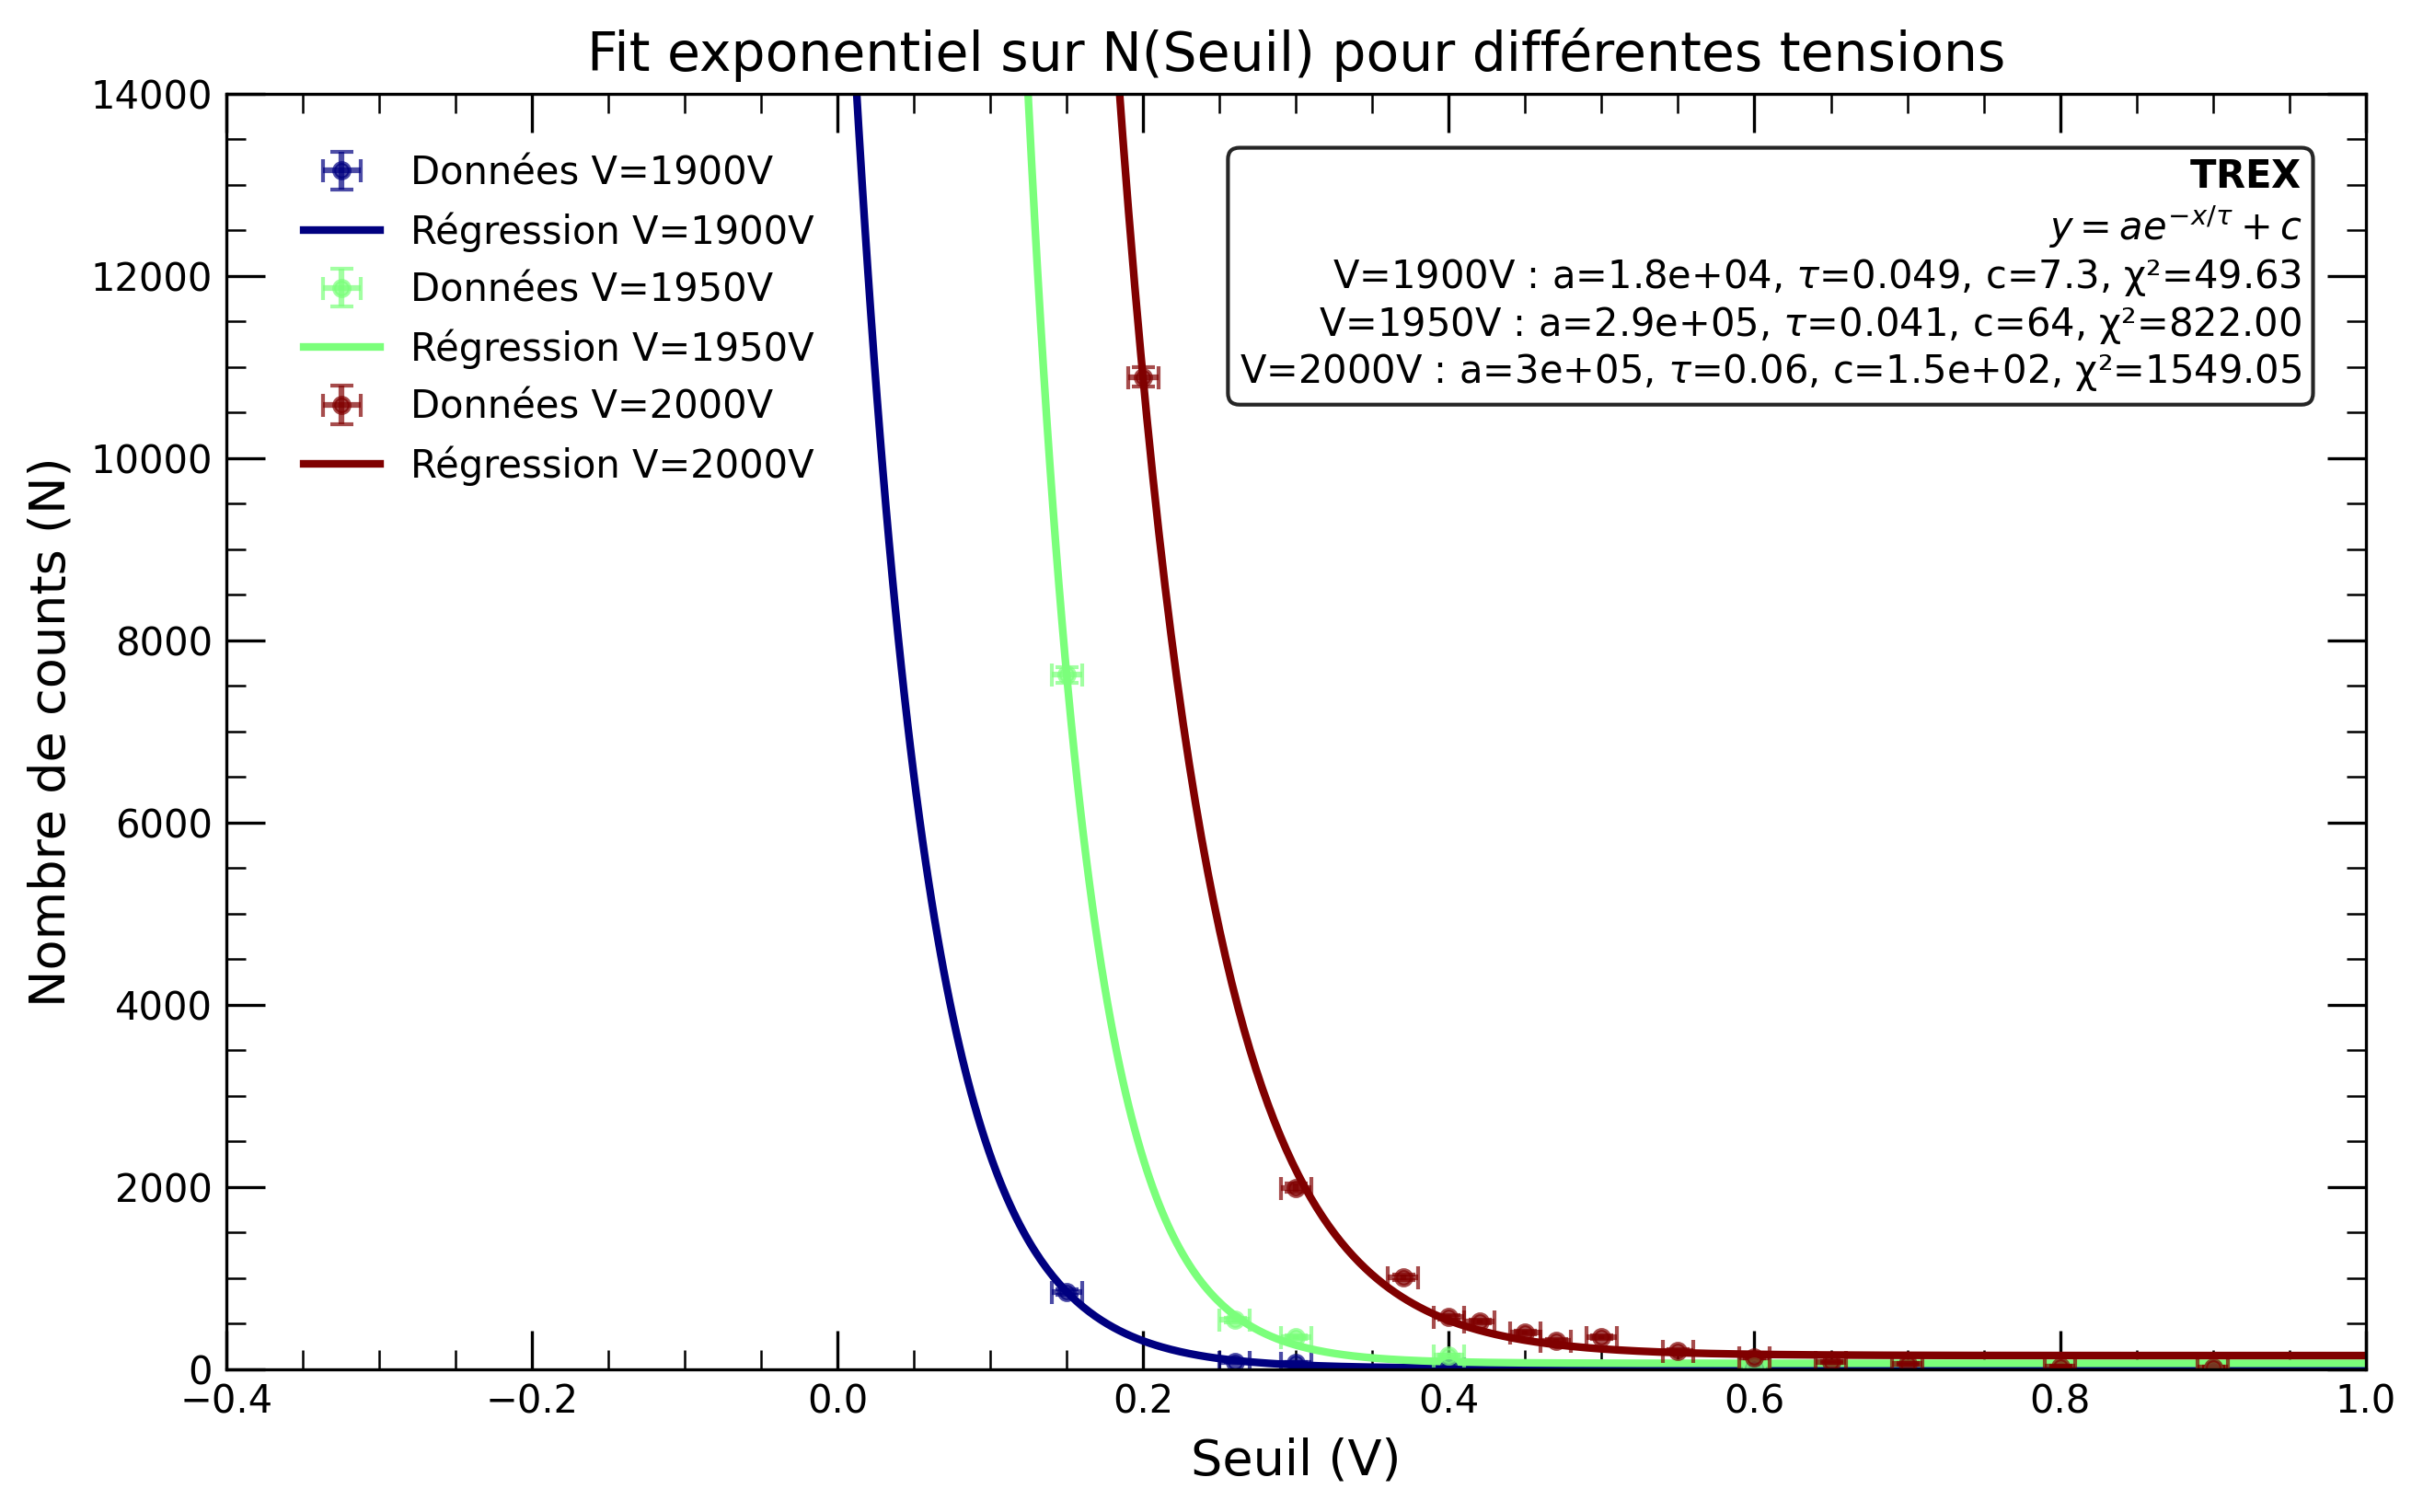
\includegraphics[width=0.9\textwidth]{Images/Threshold_Scintillateur_3.png}
    \caption{Nombre d’événements détectés en fonction du seuil pour différentes HT (Scintillateur 3).}
    \label{fig:optimisation_scint3}
\end{figure}

% --- ENCADRÉ PROBLÈMES DÉBUT ---

\vspace{1em}
\begin{center}
\begin{tcolorbox}[colback=red!5!white, colframe=red!80!black, title=Problèmes rencontrés lors de l'optimisation]
Lors de l’optimisation conjointe du seuil et de la haute tension, plusieurs difficultés majeures ont été rencontrées :
\begin{itemize}
    \item \textbf{Comptes très différents entre scintillateurs} : pour un même seuil, on observe parfois un facteur 20 entre deux scintillateurs (ex : 40 000 pour l’un, 2 000 pour l’autre).
    \item \textbf{Absence de palier net} : il était difficile d’identifier un palier clair dans la courbe de comptage ; lorsque l’on s’en approchait, le nombre de counts devenait trop faible pour modéliser correctement la zone.
    \item \textbf{Durée d’acquisition limitée} : chaque point correspond à un count par minute ; augmenter la durée pour améliorer la statistique aurait nécessité un temps d’acquisition très long (nombre de seuils $\times$ temps d’acquisition $\times$ 3 scintillateurs $\times$ nombre de tensions).
    \item \textbf{Variabilité d’un jour à l’autre} : les mesures n’étaient pas reproductibles d’un jour à l’autre, traduisant une grande sensibilité aux réglages de HT et de seuil.
\end{itemize}
Ces limitations ont rendu l’optimisation fine difficile et expliquent la dispersion des résultats.
\end{tcolorbox}
\end{center}

% --- Synthèse résultats coïncidences ---

\begin{remarque}
\textbf{Synthèse~:} Pour la coïncidence à 2 scintillateurs, la largeur de fenêtre optimale retenue est de \textbf{20 ns}, ce qui permet d’obtenir un taux de coïncidences fortuites inférieur à \textbf{10\%} du total. Pour 3 scintillateurs, une fenêtre de \textbf{20 ns} rend le taux de coïncidences fortuites négligeable (inférieur à \textbf{1\%}).

Ces résultats montrent que l’ajout d’un troisième scintillateur permet d’obtenir un signal muonique extrêmement pur, au prix d’un nombre d’événements plus faible. Le réglage fin de la fenêtre de coïncidence est donc crucial pour maximiser la pureté du signal tout en conservant une statistique exploitable.
\end{remarque}

\newpage

\section{Détection par coïncidence}

\subsection{Principe de coïncidence}

\vspace{1em}
\begin{center}
\begin{tcolorbox}[colback=blue!5!white, colframe=blue!60!black, title=Principe de la coïncidence]
Seuls les muons, très pénétrants, peuvent traverser plusieurs détecteurs alignés en quasi-ligne droite et produire des signaux quasi simultanés dans chacun. Les bruits aléatoires, eux, n’ont qu’une probabilité infime d’apparaître exactement en même temps dans deux détecteurs distincts.
\end{tcolorbox}
\end{center}

\paragraph{Pourquoi la coïncidence ?}

Dans un détecteur isolé, le taux de comptage brut inclut non seulement les événements véritables (ici des muons cosmiques traversant le scintillateur), mais aussi des détections parasites :
\begin{itemize}
    \item \textbf{Bruit thermique du photomultiplicateur} (émission spontanée d’électrons à la photocathode) ;
    \item \textbf{Radioactivité naturelle} (rayons $\gamma$ ou particules $\beta$ ambiants pouvant exciter le scintillateur) ;
    \item \textbf{Rayons cosmiques secondaires} autres que les muons (particules $\alpha$, neutrons, électrons) stoppés dans le matériau.
\end{itemize}

Pris individuellement, un scintillateur + PM peut ainsi enregistrer des comptes fictifs à un taux non négligeable. Par exemple, un photomultiplicateur à température ambiante peut avoir un bruit d’obscurité de quelques centaines de comptes par seconde. De même, l’environnement radioactif (rayonnement cosmique diffus, $\gamma$ du sol, etc.) peut induire des lueurs dans le scintillator. Il est donc essentiel de discriminer les signaux “muon” authentiques du bruit de fond.

\begin{figure}[H]
    \centering
    

% Gradient Info
  
\tikzset {_rshtctho0/.code = {\pgfsetadditionalshadetransform{ \pgftransformshift{\pgfpoint{0 bp } { 0 bp }  }  \pgftransformscale{1.8 }  }}}
\pgfdeclareradialshading{_5qzx8e19u}{\pgfpoint{0bp}{0bp}}{rgb(0bp)=(1,1,1);
rgb(0bp)=(1,1,1);
rgb(25bp)=(0,0,0);
rgb(400bp)=(0,0,0)}
\tikzset{every picture/.style={line width=0.75pt}} %set default line width to 0.75pt        

\begin{tikzpicture}[x=0.75pt,y=0.75pt,yscale=-1,xscale=1]
%uncomment if require: \path (0,300); %set diagram left start at 0, and has height of 300

%Shape: Rectangle [id:dp9388352696495245] 
\draw  [fill={rgb, 255:red, 208; green, 2; blue, 27 }  ,fill opacity=1 ] (432,48) -- (456.24,48) -- (456.24,96) -- (432,96) -- cycle ;
%Shape: Frame [id:dp16829955672449592] 
\draw   (576,0) -- (646,0) -- (646,40) -- (576,40) -- cycle(640,6) -- (582,6) -- (582,34) -- (640,34) -- cycle ;
%Shape: Rectangle [id:dp08385564233058351] 
\draw  [fill={rgb, 255:red, 74; green, 144; blue, 226 }  ,fill opacity=1 ] (467.88,48) -- (492.12,48) -- (492.12,96) -- (467.88,96) -- cycle ;
%Shape: Frame [id:dp460543295505199] 
\draw   (576,56) -- (646,56) -- (646,96) -- (576,96) -- cycle(640,62) -- (582,62) -- (582,90) -- (640,90) -- cycle ;
%Curve Lines [id:da19696877411952052] 
\draw    (528,60) .. controls (568,30) and (536.71,15.29) .. (576,24) ;
%Curve Lines [id:da024262443733791716] 
\draw    (528,72) .. controls (568,42) and (536,107) .. (576,77) ;
%Straight Lines [id:da8627449545798643] 
\draw    (456,60) -- (480,60) ;
\draw [shift={(480,60)}, rotate = 0] [color={rgb, 255:red, 0; green, 0; blue, 0 }  ][fill={rgb, 255:red, 0; green, 0; blue, 0 }  ][line width=0.75]      (0, 0) circle [x radius= 3.35, y radius= 3.35]   ;
%Straight Lines [id:da9596413715024262] 
\draw    (456,72) -- (480,72) ;
\draw [shift={(480,72)}, rotate = 0] [color={rgb, 255:red, 0; green, 0; blue, 0 }  ][fill={rgb, 255:red, 0; green, 0; blue, 0 }  ][line width=0.75]      (0, 0) circle [x radius= 3.35, y radius= 3.35]   ;
%Straight Lines [id:da8119306322827472] 
\draw    (456,84) -- (480,84) ;
\draw [shift={(480,84)}, rotate = 0] [color={rgb, 255:red, 0; green, 0; blue, 0 }  ][fill={rgb, 255:red, 0; green, 0; blue, 0 }  ][line width=0.75]      (0, 0) circle [x radius= 3.35, y radius= 3.35]   ;
%Shape: Rectangle [id:dp3987182356264175] 
\draw  [fill={rgb, 255:red, 144; green, 19; blue, 254 }  ,fill opacity=1 ] (503.76,48) -- (528,48) -- (528,96) -- (503.76,96) -- cycle ;
%Straight Lines [id:da6712190365201196] 
\draw    (480,72) -- (516,72) ;
\draw [shift={(516,72)}, rotate = 0] [color={rgb, 255:red, 0; green, 0; blue, 0 }  ][fill={rgb, 255:red, 0; green, 0; blue, 0 }  ][line width=0.75]      (0, 0) circle [x radius= 3.35, y radius= 3.35]   ;
%Straight Lines [id:da780749344939817] 
\draw    (480,84) -- (516,72) ;
\draw [shift={(516,72)}, rotate = 341.57] [color={rgb, 255:red, 0; green, 0; blue, 0 }  ][fill={rgb, 255:red, 0; green, 0; blue, 0 }  ][line width=0.75]      (0, 0) circle [x radius= 3.35, y radius= 3.35]   ;
%Straight Lines [id:da7632950645361253] 
\draw    (480,60) -- (516,72) ;
\draw [shift={(516,72)}, rotate = 18.43] [color={rgb, 255:red, 0; green, 0; blue, 0 }  ][fill={rgb, 255:red, 0; green, 0; blue, 0 }  ][line width=0.75]      (0, 0) circle [x radius= 3.35, y radius= 3.35]   ;
%Rounded Rect [id:dp0463394923852084] 
\path  [shading=_5qzx8e19u,_rshtctho0] (300,60) .. controls (300,55.58) and (303.58,52) .. (308,52) -- (412,52) .. controls (416.42,52) and (420,55.58) .. (420,60) -- (420,84) .. controls (420,88.42) and (416.42,92) .. (412,92) -- (308,92) .. controls (303.58,92) and (300,88.42) .. (300,84) -- cycle ; % for fading 
 \draw   (300,60) .. controls (300,55.58) and (303.58,52) .. (308,52) -- (412,52) .. controls (416.42,52) and (420,55.58) .. (420,60) -- (420,84) .. controls (420,88.42) and (416.42,92) .. (412,92) -- (308,92) .. controls (303.58,92) and (300,88.42) .. (300,84) -- cycle ; % for border 

%Straight Lines [id:da13295955815022265] 
\draw    (420,72) -- (432,72) ;

% Text Node
\draw (580,11) node [anchor=north west][inner sep=0.75pt]   [align=left] {{\tiny \textbf{Oscilloscope}}};
% Text Node
\draw (417,31.2) node [anchor=north west][inner sep=0.75pt]   [align=left] {{\tiny Amplificateur}};
% Text Node
\draw (445,98) node [anchor=north west][inner sep=0.75pt]   [align=left] {{\tiny Discriminateur}};
% Text Node
\draw (590,73) node [anchor=north west][inner sep=0.75pt]  [font=\footnotesize] [align=left] {{\fontfamily{pcr}\selectfont {\footnotesize \textcolor[rgb]{1,0,0}{000}}}};
% Text Node
\draw (619,72) node [anchor=north west][inner sep=0.75pt]  [font=\footnotesize] [align=left] {{\fontfamily{pcr}\selectfont {\tiny \textcolor[rgb]{1,0,0}{600s}}}};
% Text Node
\draw (584,63) node [anchor=north west][inner sep=0.75pt]   [align=left] {{\tiny \textbf{Compteur}}};
% Text Node
\draw (485.4,23) node [anchor=north west][inner sep=0.75pt]   [align=left] {{\tiny Coincidences }};
% Text Node
\draw (505.4,30) node [anchor=north west][inner sep=0.75pt]   [align=left] {{\tiny unit}};

% Text Node
\draw (577,44) node [anchor=north west][inner sep=0.75pt]   [align=left] {{\tiny Coincidences }};
% Text Node
\draw (304,61) node [anchor=north west][inner sep=0.75pt]   [align=left] {{\tiny Ensemble scintillateurs}};
% Text Node
\draw (304,70) node [anchor=north west][inner sep=0.75pt]   [align=left] {{\tiny  PMT, HT}};
% Text Node




\end{tikzpicture}

    \caption{Montage electronique de coïncidence avec les scintillateurs.}
    \label{fig:coincidence_sans_delais}
\end{figure}

\begin{figure}[H]
    \centering
    %\includegraphics[width=0.6\textwidth]{figures/schema_coincidence.pdf}
    \fbox{\parbox{0.6\textwidth}{\centering\textit{Schéma à insérer : deux scintillateurs A et B alignés, un muon traverse les deux, signaux synchrones. Les bruits parasites (étoiles, zigzags) ne traversent qu'un seul détecteur à la fois.}}}
    \caption{Principe de la coïncidence temporelle : seuls les muons traversent les deux détecteurs en même temps.}
\end{figure}

% --- 4.2 Principe des coïncidences fortuites ---

\newpage

\subsection{Principe des coïncidences fortuites}

\begin{center}
\begin{tcolorbox}[colback=blue!5!white, colframe=blue!60!black, title=Principe des coïncidences fortuites]
Même si la probabilité est faible, il peut arriver que deux signaux indépendants (issus du bruit de fond, de la radioactivité ou du bruit électronique) surviennent par hasard dans la même fenêtre temporelle de coïncidence. Le module de coïncidence les interprète alors à tort comme le passage d’un muon, alors qu’il s’agit d’un événement purement fortuit.
\end{tcolorbox}
\end{center}

Nous avons aussi estimé le nombre de coïncidences fortuites, c’est-à-dire les coïncidences dues au bruit et non aux muons. Pour cela, nous avons utilisé la méthode du délai (delay) :

\begin{itemize}
    \item \textbf{Pour 2 scintillateurs}~: nous avons introduit un délai sur l’un des deux signaux avant son entrée dans le module de coïncidence. En choisissant un délai supérieur à la fenêtre temporelle (width) de la coïncidence, on s’assure que les impulsions issues d’un même muon ne peuvent plus être détectées simultanément. Ainsi, tous les événements enregistrés dans cette configuration sont nécessairement des coïncidences fortuites, c’est-à-dire dues à des bruits indépendants sur chaque détecteur. Le nombre de coïncidences mesuré avec ce décalage donne donc directement le taux de fond accidentel.
    \item \textbf{Pour 3 scintillateurs}~: la même logique a été appliquée, mais cette fois en introduisant deux délais différents sur deux des trois signaux. Cela garantit qu’aucun muon ne peut produire une triple coïncidence réelle, et que tous les événements enregistrés sont fortuits. On mesure alors en parallèle le nombre de coïncidences avec et sans délai~: la différence entre les deux donne le nombre de “vrais” muons détectés, c’est-à-dire le signal purifié du bruit de fond.
\end{itemize}

Cette méthode permet donc d’estimer précisément la pureté du signal et de quantifier la part de coïncidences réellement attribuables au passage de muons, en soustrayant le fond mesuré avec délai au signal total.

\newpage

\subsection{Résultats expérimentaux}
\subsubsection{Coïncidence à 2 scintillateurs}

Le graphique ci-dessous présente, pour le couple de scintillateurs 1 et 2, les résultats obtenus avec un seuil de 0{,}45~V et une haute tension de 2000~V pour le scintillateur 1, et un seuil de 0{,}05~V et une haute tension de 1950~V pour le scintillateur 2 (valeurs optimisées à partir des expériences précédentes).

Pour chaque largeur de fenêtre de coïncidence (width), on a mesuré :
\begin{itemize}
    \item le nombre total de coïncidences enregistrées en 4 minutes (sans délai)~;
    \item le nombre de coïncidences fortuites (avec un délai de 63~ns appliqué sur l’un des signaux, ce qui supprime les vraies coïncidences muoniques)~;
    \item la différence entre les deux, qui correspond au nombre de “vrais” muons détectés.
\end{itemize}

On observe que lorsque la fenêtre de coïncidence est large, le nombre de coïncidences fortuites augmente fortement, tandis que pour des fenêtres plus étroites, la proportion de vrais muons devient dominante. Ce protocole permet donc d’optimiser le réglage du width pour maximiser la pureté du signal muonique tout en conservant un nombre d’événements suffisant.


\begin{figure}[H]
    \centering
    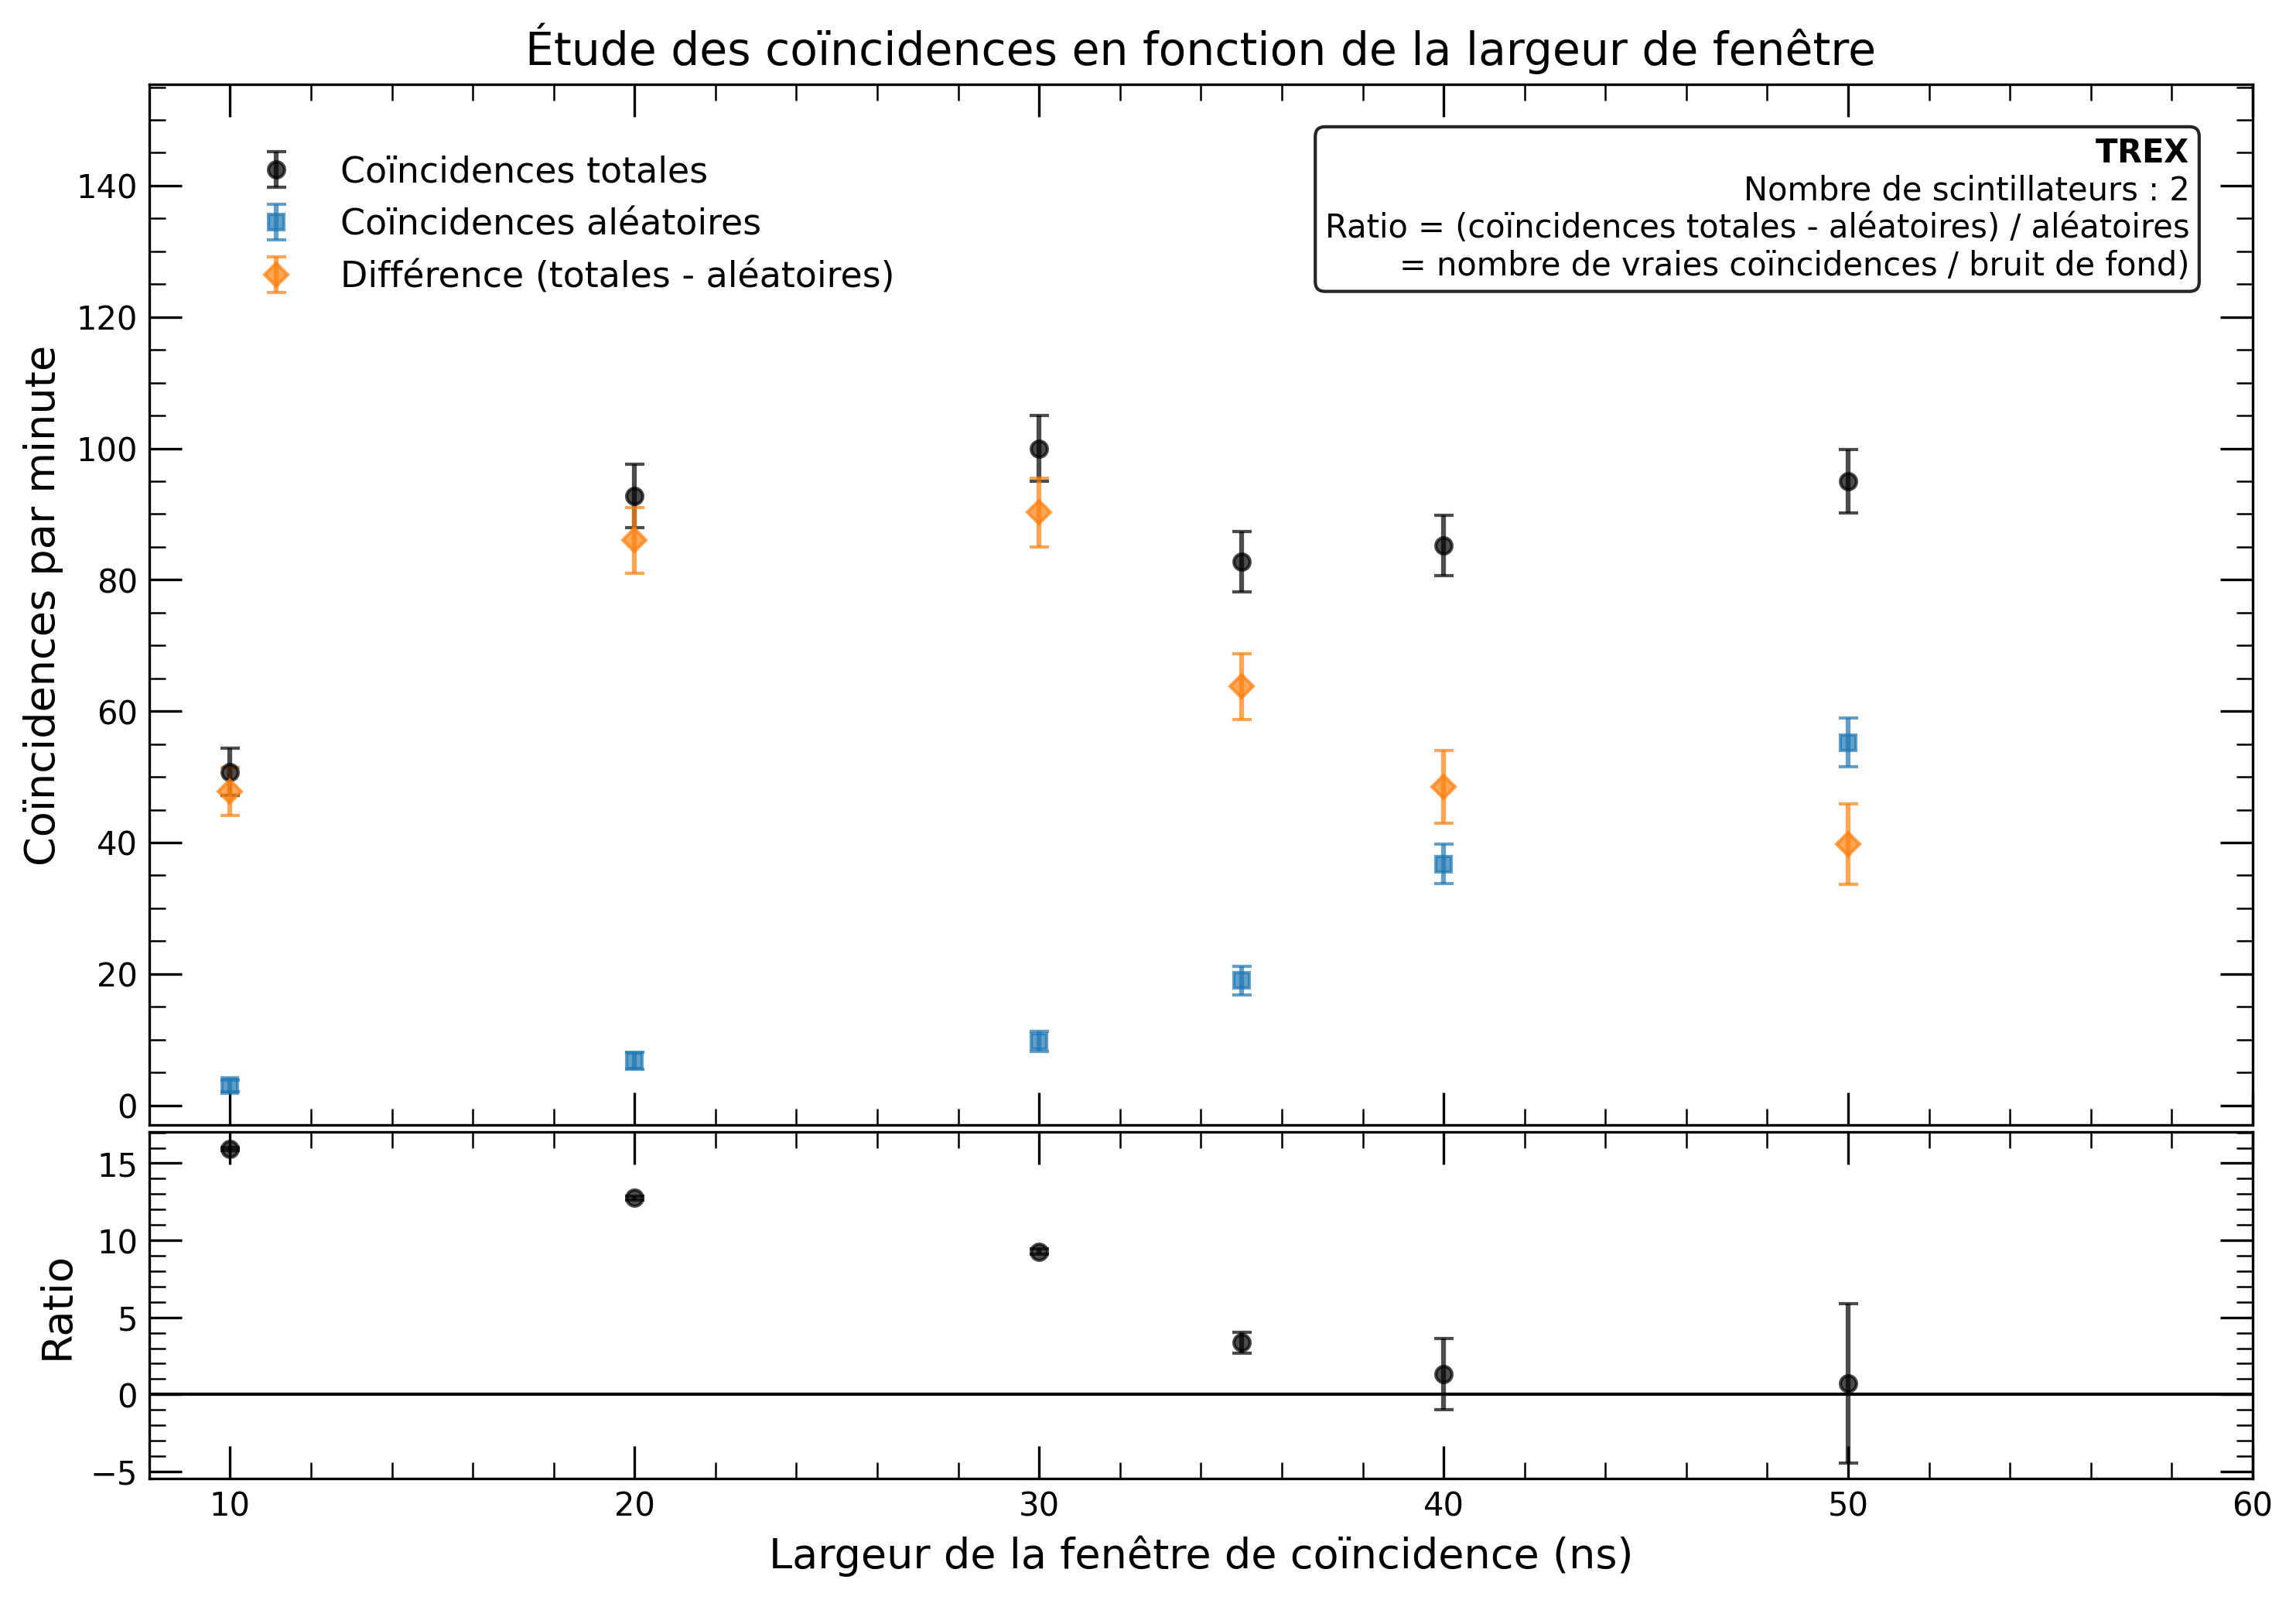
\includegraphics[width=0.9\textwidth]{Images/Coincidences_2_Scintillateurs.png}
    \caption[Nombre d’évènement en 4 min en fonction du seuil]{Nombre d’évènement en 4min en fonction du seuil pour 2 scintillateurs en coïncidence}
\end{figure}

Enfin, l’ordre de grandeur de détection est à présent de 100 coïncidences par sec par m$^2$, qui correspond bien à l’ordre de grandeur attendu.

\subsubsection{Coïncidence à 3 scintillateurs}

Le graphique ci-dessous présente les résultats obtenus pour la coïncidence à 3 scintillateurs, avec les réglages suivants :
\begin{itemize}
    \item Scintillateur 1 : seuil de 0{,}45~V, haute tension de 2000~V
    \item Scintillateur 2 : seuil de 0{,}05~V, haute tension de 2050~V, delay = 63~ns
    \item Scintillateur 3 : seuil de 0{,}3~V, haute tension de 2060~V, delay = 31~ns
\end{itemize}
Ces valeurs ont été choisies à partir des optimisations précédentes.

Pour chaque largeur de fenêtre de coïncidence (width), on a mesuré :
\begin{itemize}
    \item le nombre total de coïncidences enregistrées en 10 minute (sans délai)~;
    \item le nombre de coïncidences fortuites (avec deux délais appliqués sur les signaux des scintillateurs 2 et 3, supprimant ainsi les vraies coïncidences muoniques)~;
    \item la différence entre les deux, qui correspond au nombre de “vrais” muons détectés~;
    \item le ratio entre le nombre de vraies coïncidences et le nombre de coïncidences fortuites, indicateur direct de la pureté du signal.
\end{itemize}

On constate que l’utilisation de trois scintillateurs permet de réduire drastiquement le nombre de coïncidences fortuites, et que le ratio signal/bruit devient très élevé pour des fenêtres de coïncidence raisonnables. Ce protocole permet donc d’obtenir un signal muonique extrêmement pur, au prix d’un nombre d’événements plus faible.

\begin{figure}[H]
    \centering
    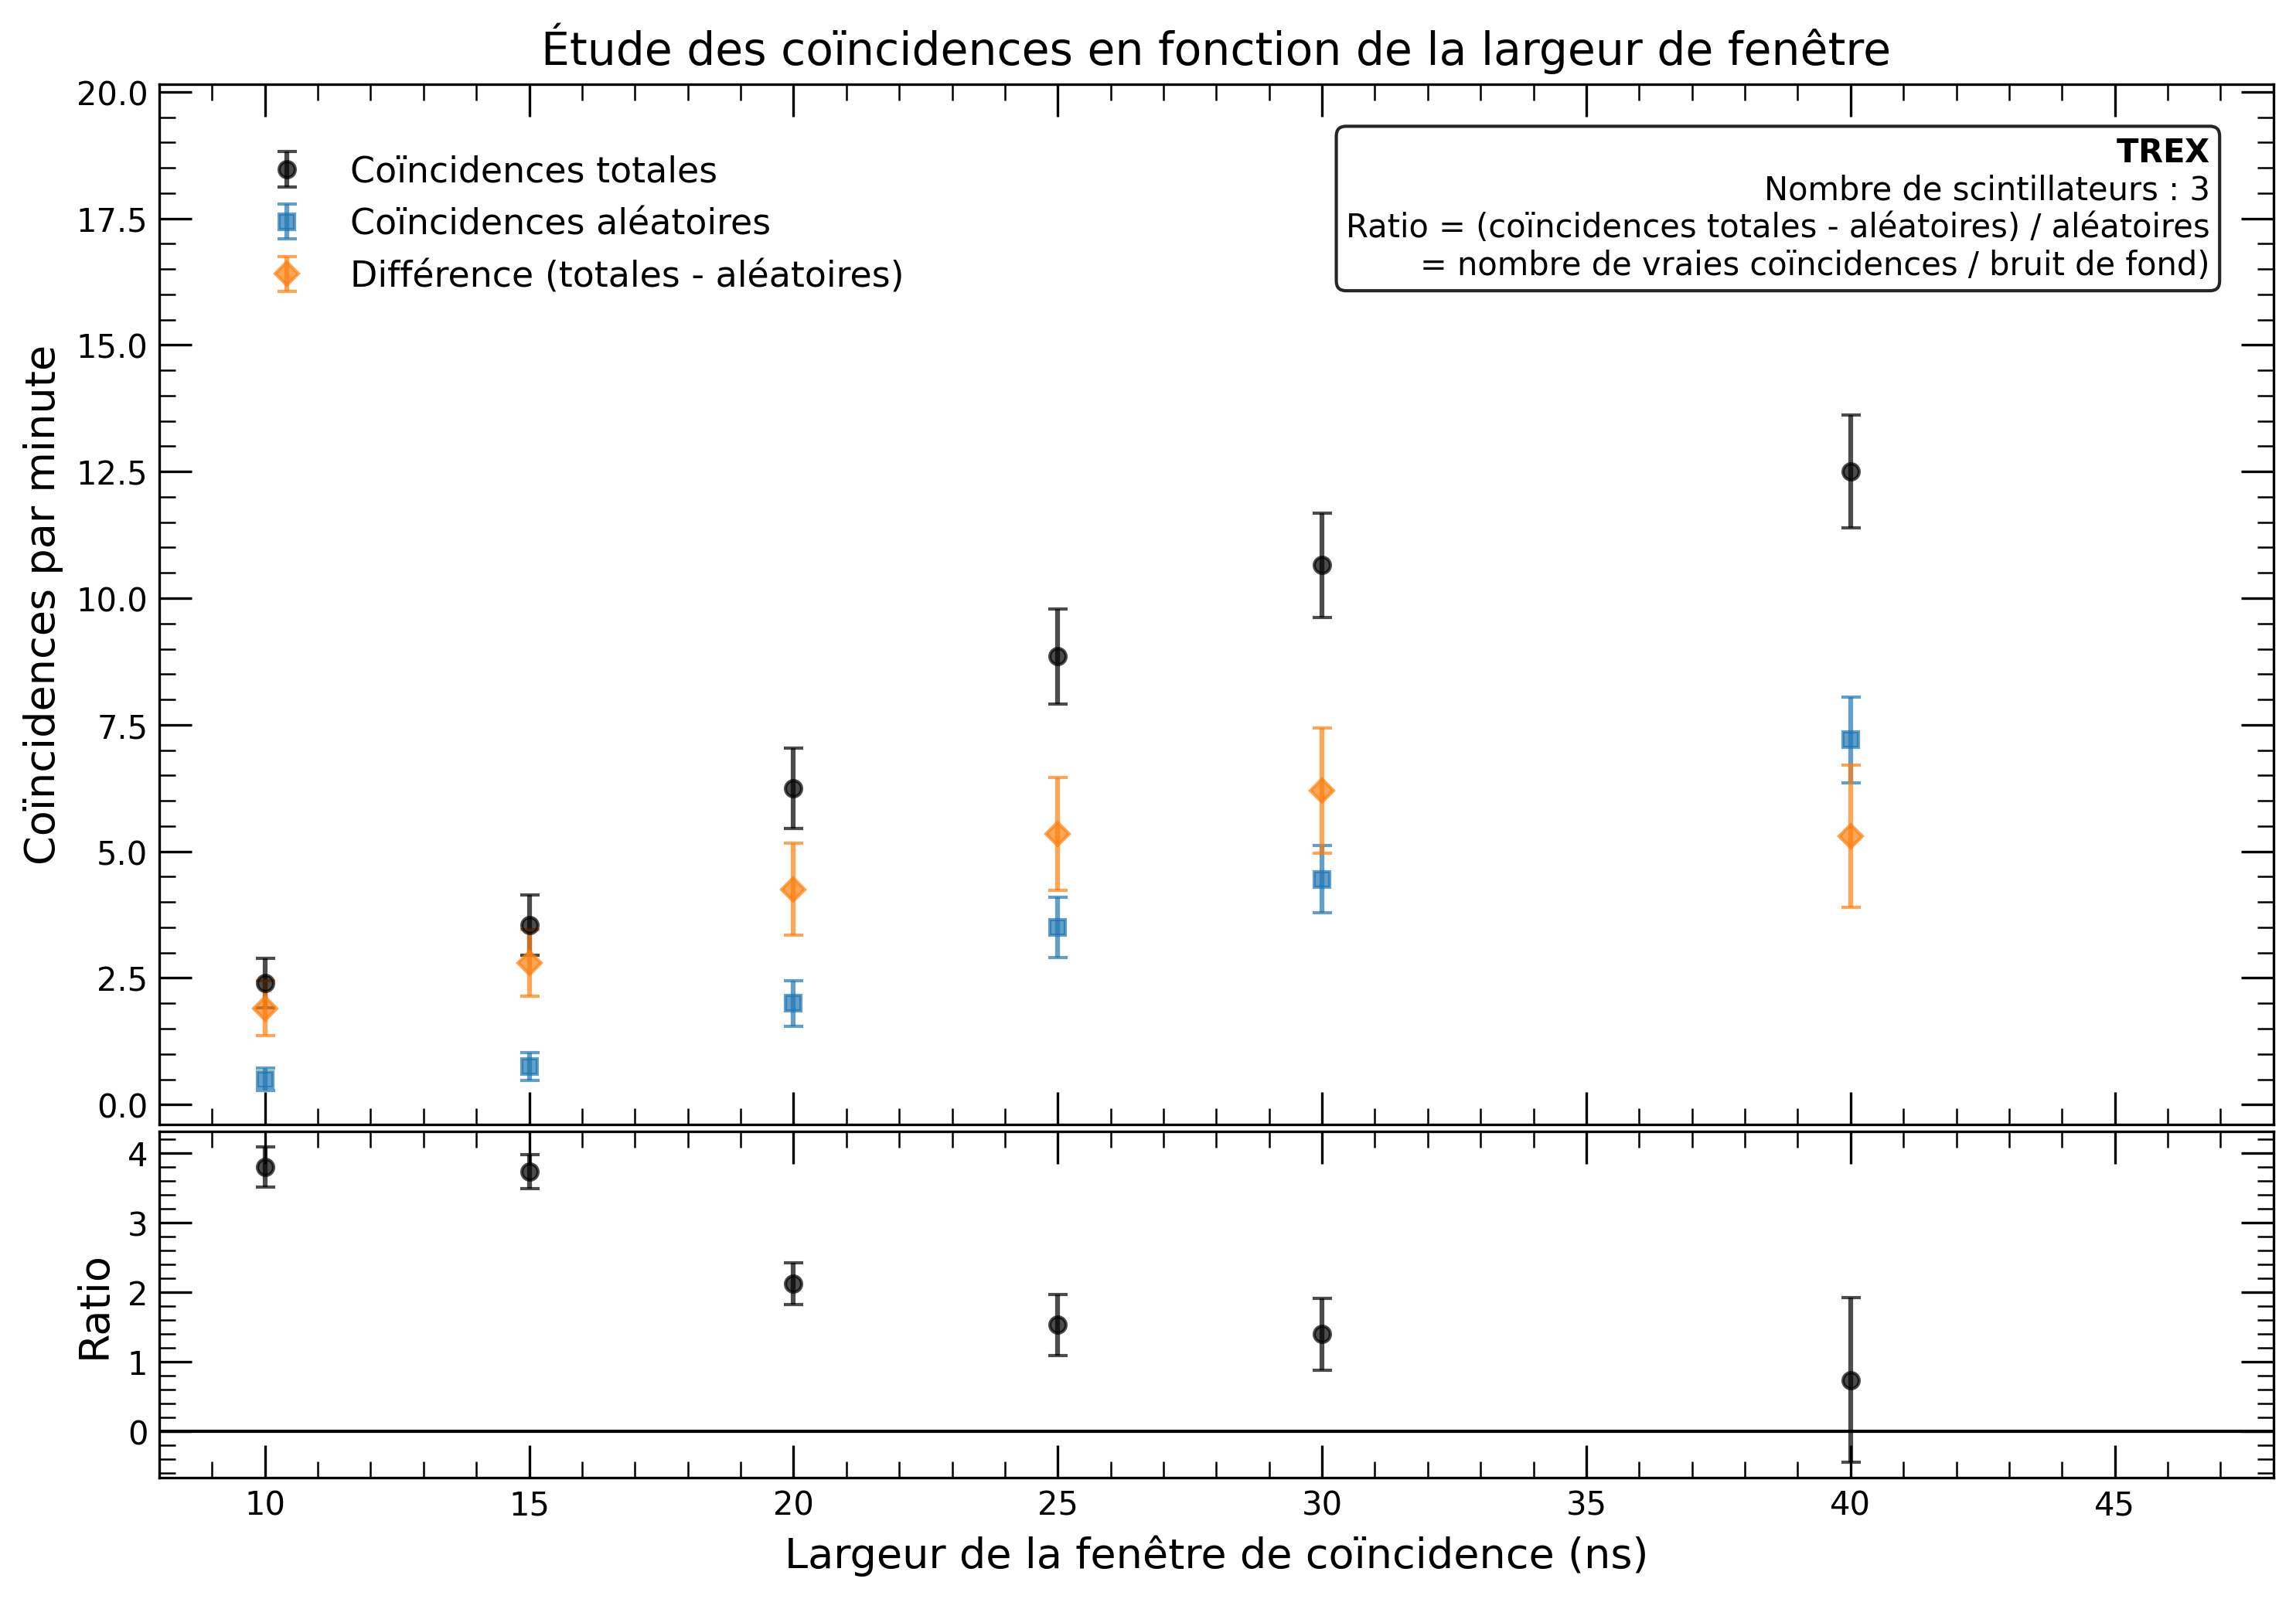
\includegraphics[width=0.9\textwidth]{Images/Coincidences_3_Scintillateurs.png}
    \caption[Nombre d’évènement en 4min en fonction du seuil]{Nombre d’évènement en 10 min en fonction du seuil pour 3 scintillateurs en coïncidence}
\end{figure}

% --- Encadré Problèmes rencontrés lors des mesures de coïncidences ---

\vspace{1em}
\begin{center}
\begin{tcolorbox}[colback=red!5!white, colframe=red!80!black, title=Problèmes rencontrés lors des mesures de coïncidences]
Lors des mesures de coïncidences (notamment à 3 scintillateurs), plusieurs difficultés majeures ont été rencontrées :
\begin{itemize}
    \item \textbf{Nombre de coïncidences très faible} : surtout avec 3 scintillateurs, le taux de coïncidences était très bas, nécessitant des temps d'acquisition très longs (parfois 10 minutes par point), ce qui a rendu les manipulations longues et sujettes à de grandes incertitudes statistiques.
    \item \textbf{Différences entre scintillateurs} : le nombre de coïncidences à 2 scintillateurs dépendait fortement de la paire choisie, les scintillateurs étant très différents en efficacité. De nombreux tests ont été nécessaires pour choisir la meilleure combinaison.
    \item \textbf{Retard dans les câbles} : le retard dû à la longueur des câbles diffère selon le scintillateur. Nous avons supposé cet effet négligeable, mais il a pu influencer les mesures.
\end{itemize}
Ces limitations ont rendu l’optimisation fine difficile et expliquent la dispersion des résultats.
\end{tcolorbox}
\end{center}

% --- Synthèse résultats coïncidences ---

\begin{remarque}
\textbf{Synthèse~:} Pour la coïncidence à 2 scintillateurs, la largeur de fenêtre optimale retenue est de \textbf{20 ns}, ce qui permet d’obtenir un taux de coïncidences fortuites inférieur à \textbf{10\%} du total. Pour 3 scintillateurs, une fenêtre de \textbf{20 ns} rend le taux de coïncidences fortuites négligeable (inférieur à \textbf{1\%}).

Ces résultats montrent que l’ajout d’un troisième scintillateur permet d’obtenir un signal muonique extrêmement pur, au prix d’un nombre d’événements plus faible. Le réglage fin de la fenêtre de coïncidence est donc crucial pour maximiser la pureté du signal tout en conservant une statistique exploitable.
\end{remarque}

\newpage

\section{Distribution angulaire du flux muonique}
L'un des caract\`eres notables du rayonnement cosmique muonique au niveau du sol est son anisotropie en angle \text{\'enithal}. Les muons proviennent majoritairement de la verticale, c'est-\`a-dire de la direction du \text{\'enith} (car ils sont g\'en\'er\'es en haute atmosph\`ere et suivent grossi\`erement des trajectoires quasi-rectilignes vers le bas). Plus l'angle~$\theta$ par rapport \`a la verticale augmente (muons venant rasants de l'horizon), plus le parcours dans l'atmosph\`ere est long, et donc plus la probabilit\'e de survie du muon jusqu'au sol diminue. Ce ph\'enom\`ene se traduit par une loi empirique proche de
\[
  I(\theta) = I(0)\cos^n\theta,
\]
avec $n \approx 2$ aux 'energies cosmiques typiques. Autrement dit, le flux diff\'erentiel de muons est approximativement proportionnel \`a $\cos^2\theta$ pour des angles mod\'er\'es. Des mesures plus fines montrent qu'\`a tr\`es grands angles ($\theta > 60^\circ$), la distribution s'att\'enue plus fortement que le simple $\cos^2$ en raison de la courbure terrestre (au-del\`a d'un certain angle, les muons provenant de l'horizon ont parcouru une distance atmosph\`erique si grande qu'aucun n'atteint le sol) et de la s\'election en 'energie (seuls les muons les plus 'energiques arrivent depuis des angles rasants sans se d\'esint\'egrer). N\'eanmoins, dans l'intervalle $0^\circ \le \theta \leq 60^\circ$, on peut consid\'erer la loi $\cos^2\theta$ comme une bonne approximation pour le flux muonique au niveau de la mer.

\newpage

\subsection{Mise en œuvre expérimentale}
Pour chaque angle~$\theta$, on enregistre le nombre de muons détectés (coïncidences $A\wedge B$) pendant une durée fixe (par ex.\ quelques minutes, suffisamment pour accumuler des centaines d’événements et réduire l’erreur statistique). On obtient ainsi un taux de comptage~$N(\theta)$ en fonction de~$\theta$. Les résultats bruts doivent être corrigés de deux effets géométriques~: (i) la projection de la surface du détecteur selon l'angle, et (ii) l'acceptation commune des deux plaques (qui varie légèrement avec l'angle dans notre montage). Le premier point est important~: lorsque le télescope est incliné de~$\theta$, la surface effective présentée aux muons venant du zénith est réduite d'un facteur~$\cos\theta$. Inversement, pour des muons venant réellement d'une direction inclinée~$\theta$, la surface présentée est maximale. En pratique, pour relier au flux angulaire~$I(\theta)$ (défini par unité de surface perpendiculaire à la direction d'arrivée), il faut diviser le taux mesuré par~$\cos\theta$ (correction de projection). Le second point concerne la portion de ciel vue par les deux détecteurs en coïncidence~: dans notre cas, pour des angles modérés, on peut considérer qu'elle reste constante tant que la superposition des deux scintillateurs est complète.

Après ces corrections, on peut comparer la distribution normalisée~$I_{\mathrm{mesure}}(\theta)$ au modèle en~$\cos^{2}\theta$. Les données obtenues présentent une bonne conformité avec la loi attendue. Graphique~1 ci‑dessous montre, de façon qualitative, la tendance mesurée~: en représentant $N(\theta)$ corrigé en fonction de~$\cos\theta$, on obtient approximativement une droite, ce qui traduit
\[
N(\theta)\propto\cos^{2}\theta.
\]
Plus précisément, un ajustement polynomial donne une puissance~$n$ très proche de~2 pour la dépendance en cosinus. Par exemple, nos mesures indiquent un rapport
\[
\frac{N(60^\circ)}{N(0^\circ)} \approx \bigl(\cos 60^\circ\bigr)^2 = 0{,}25,
\]
en accord avec la loi~$\cos^2$ (compte tenu des incertitudes). Pour $\theta$ au‑delà de~70--$80^\circ$, le signal devient difficile à mesurer (très faible) et dévie de la simple loi~$\cos^2$ (chute plus rapide), cohérent avec l'atténuation atmosphérique supplémentaire non prise en compte par le modèle simplifié.

Interprétation~: la loi $I(\theta)\propto\cos^2\theta$ résulte de la combinaison de deux effets principaux.  
(i) Distribution isotrope à la production~: les pions parents des muons sont produits isotropiquement dans le référentiel du laboratoire (en première approximation), et leur désintégration donne des muons distribués également dans l'espace (avec un léger biais avant, négligeable ici). Ainsi, le flux de muons incident sur la Terre en l'absence d'atmosphère serait isotrope, donc $\propto\cos\theta$ simplement à cause de la projection de surface.  
(ii) Parcours atmosphérique variable~: les muons créés à un angle~$\theta$ doivent traverser une épaisseur d'atmosphère $X(\theta)$ plus grande que ceux venant du zénith. Pour un angle zénithal~$\theta$, la colonne d'air parcourue est approximativement
\[
X(\theta)=\frac{X(0)}{\cos\theta}
\]
(pour $\theta$ pas trop grand et en négligeant la courbure terrestre), où $X(0)$ est l'épaisseur verticale correspondant à 1013 hPa (environ 1030 g/$cm^2$ d'équivalent masse d'air). La probabilité de survie d'un muon jusqu'au sol décroît exponentiellement avec~$X$:
\[
P_{\mathrm{survie}}(\theta)\approx\exp\bigl(-X(\theta)/\Lambda_{\mu}\bigr),
\]
avec $\Lambda_{\mu}$ la longueur d'atténuation (liée à la longueur de désintégration $\gamma c\tau$ des muons, de l'ordre de~6 km d'équivalent air pour des muons de quelques GeV). Pour des angles modérés, on peut développer à premier ordre :
\[
P(\theta)\approx \exp\!\Bigl(-\bigl(\tfrac{X(0)}{\Lambda_\mu}\bigr)\bigl(\tfrac1{\cos\theta}-1\bigr)\Bigr)\approx \exp\!\Bigl(-\bigl(\tfrac1{\cos\theta}-1\bigr)\tfrac{X(0)}{\Lambda_\mu}\Bigr).
\]
Si $\tfrac{X(0)}{\Lambda_\mu}$ n'est pas trop grand (typiquement 1--3), on peut approximer 
\[
\exp\!\Bigl(-\bigl(\tfrac1{\cos\theta}-1\bigr)\tfrac{X(0)}{\Lambda_\mu}\Bigr)\sim\cos^n\theta
\]
pour un certain~$n$. Les valeurs réalistes donnent effectivement un $n\approx2$. Intuitivement, on combine cette atténuation en~$\cos\theta$ avec le facteur géométrique $\cos\theta$ d'un flux isotrope, ce qui produit $\cos^2\theta$ au total. En réalité, le spectre en énergie entre aussi en jeu : les muons plus inclinés doivent avoir une énergie plus grande pour survivre (sinon ils se désintègrent en route), ce qui modifie légèrement l'exposant~$n$ en fonction du seuil d'énergie considéré.

Nos résultats expérimentaux confirment donc bien la diminution du flux de muons cosmiques aux grands angles. Cette anisotropie est en accord avec la compréhension actuelle des gerbes atmosphériques : les muons proviennent majoritairement des pions produits à une altitude d’environ 15 km et voyageant vers le sol. Le fait qu’on observe encore des muons à des angles assez rasants illustre leur grande énergie initiale et la dilatation du temps de vie (sans relativité, aucun muon formé à 15 km ne pourrait parcourir plus de 600 m avant de se désintégrer, et ne parviendrait pas jusqu’à nous). Ces mesures angulaires rejoignent des observations globales : par exemple, en intégrant sur tous les angles, on trouve un flux global d’environ $170\text{muons}/\text{m}^2/\text{s}$ au niveau de la mer, dont la composante quasi-horizontale est très minoritaire.

En conclusion de cette partie, la mise en évidence expérimentale de la loi en $\cos^2\theta$ est une validation importante. Notre télescope à scintillateurs, en dépit de sa simplicité, a permis de cartographier l’intensité du rayonnement cosmique selon l’angle, en bon accord avec le modèle théorique. Cela illustre la nécessité de corriger de la projection géométrique lorsqu’on compare des taux de comptage entre configurations inclinées, et met en avant l’influence de l’absorption atmosphérique sur les particules cosmiques secondaires.

% --- Encadré Problèmes rencontrés lors de la mesure angulaire ---

\vspace{1em}
\begin{center}
\begin{tcolorbox}[colback=red!5!white, colframe=red!80!black, title=Problèmes rencontrés lors de la mesure angulaire]
Les trois scintillateurs utilisés ne sont pas récents, et la surface d’un scintillateur n’absorbe pas uniformément sur toute sa surface. Ainsi, lorsque l’on incline les scintillateurs pour mesurer sous différents angles, la zone d’intersection peut se trouver sur des parties plus ou moins usées ou moins efficaces. Cela introduit une incertitude supplémentaire sur les mesures, car la réponse dépend localement de l’état d’usure et d’efficacité de chaque scintillateur.
\end{tcolorbox}
\end{center}

\newpage

\section{Mesure de l’énergie d’un muon}
Les muons cosmiques arrivant au sol possèdent un spectre continu d’énergies s’étendant de centaines de MeV à plusieurs dizaines de GeV. Leur énergie moyenne est d’environ 3–4 GeV, et un grand nombre sont minimisants (c’est-à-dire déposent l’énergie minimum par unité de longueur dans la matière, comme des particules traversant vite sans se freiner complètement). Dans cette section, nous cherchons à caractériser expérimentalement la manière dont les muons interagissent avec la matière, en particulier en observant combien d’énergie ils déposent dans le détecteur et comment un absorbeur de plomb placé sur leur trajectoire affecte le comptage.

\begin{itemize}
  \item Dépôt d’énergie dans le scintillateur : distribution de Landau.
  \item Expérience avec absorbeur de plomb : pertes par ionisation, bremsstrahlung et capture.
  \item Analyse des effets expérimentaux : baisse de 15\% du taux de coïncidence, augmentation du dépôt d’énergie moyen.
\end{itemize}

Dépôt d’énergie dans le scintillator (spectre de Landau) : Lorsqu’un muon traverse un scintillateur de épaisseur donnée, l’énergie qu’il y perd par ionisation fluctue d’un événement à l’autre. Ces fluctuations de $dE$ proviennent de processus stochastiques : un muon peut perdre un peu plus d’énergie s’il crée un delta-ray (électron secondaire de haute énergie) ou un peu moins s’il traverse sans collision violente. La distribution théorique du dépôt d’énergie dans une mince couche de matière est décrite par la statistique de Landau (distribution de Landau), caractérisée par un pic le plus probable et une longue traîne vers les hautes énergies perdues. Typiquement, pour un muon minimum ionisant traversant ~1 cm de plastique (1–1,2 g/cm²), le dépôt d’énergie le plus probable est de l’ordre de 1–2 MeV, alors que la moyenne de la distribution est légèrement supérieure (quelques MeV) en raison de la contribution de la traîne. Dans notre détecteur, cette énergie déposée se traduit en un nombre de photons scintillants puis en une amplitude de signal PM proportionnelle. En enregistrant ces amplitudes (via un multi-channel analyzer par exemple), on pourrait observer le spectre d’énergie déposée : on s’attend à un pic de Landau assez large centré aux alentours de 1–2 MeV, avec une queue étendue jusqu’à peut-être 5–10 MeV due aux pertes occasionnelles plus importantes.

Dans le cadre de cette expérience, plutôt que de mesurer directement le spectre d’amplitude (ce qui nécessiterait un spectromètre d’amplitude calibré), nous avons étudié le dépôt d’énergie de manière indirecte en examinant l’effet d’un absorbeur sur le taux de comptage et sur le signal.

Expérience avec absorbeur de plomb : Nous avons inséré une plaque de plomb de 5 cm d’épaisseur au-dessus du scintillateur supérieur du télescope, de sorte que les muons devaient traverser ce blindage avant d’entrer dans les scintillateurs. Le plomb, matériau de numéro atomique élevé (Z=82) et de densité $\rho \approx 11,3$ g/cm³, sert de filtre absorbant : il va ralentir les muons en leur faisant perdre de l’énergie supplémentaire, et potentiellement en arrêter certains. Plusieurs phénomènes se produisent lorsqu’un muon traverse du plomb :
	•	Perte d’énergie par ionisation accrue : La densité élevée fait qu’en 5 cm de Pb (soit ~56,5 g/cm²), un muon va perdre environ $\Delta E \approx (dE/dx) \times 56,5$ g/cm². Pour un muon minimum ionisant, $dE/dx \sim 1,5 - 2$ MeV·cm²/g dans le plomb (valeur typique dans les métaux), donc $\Delta E \sim 85$ à 110 MeV. Ainsi, un muon doit avoir au moins ~100 MeV d’énergie cinétique pour traverser cette épaisseur de plomb. Or pratiquement tous les muons cosmiques atteignant le sol ont bien plus que 100 MeV (puisque déjà 2 GeV sont perdus dans l’atmosphère). Donc la plupart des muons ne seront pas complètement arrêtés par 5 cm de plomb ; ils en ressortiront simplement un peu moins énergétiques (par exemple, un muon de 1 GeV ressort à ~0,9 GeV).
	•	Production de rayonnement de freinage (bremsstrahlung) et secondaires : Un muon de plusieurs GeV traversant du plomb peut, s’il interagit avec le champ coulombien des noyaux, émettre un photon gamma de bremsstrahlung ou produire un changement de régime pour des énergies extrêmes. Cependant, le muon étant ~200 fois plus lourd que l’électron, le rayonnement de freinage est fortement supprimé par rapport à un électron. En dessous de plusieurs centaines de GeV, le mécanisme dominant de perte reste l’ionisation. Donc pour nos énergies (quelques GeV au plus), la contribution radiative dans 5 cm de plomb est mineure. Il peut y avoir création de quelques électrons δ (delta) dans le plomb, qui eux-mêmes pourraient donner un surcroît de lumière s’ils atteignent le scintillator.
	•	Arrêt et capture des muons lents : Si un muon initialement peu énergétique (disons ~0,2–0,3 GeV) arrive dans le plomb, il se peut qu’il s’y arrête entièrement. Un muon stoppé dans le plomb (surtout s’il est μ⁻) a une probabilité de se faire capturer par un noyau de plomb (capture muonique) au lieu de se désintégrer, ce qui le fait disparaître sans émettre le signal attendu dans le scintillateur. Cependant, étant donné le spectre des muons cosmiques (très peu ont <300 MeV en arrivant au sol, car les moins énergétiques ont déjà majoritairement désintégré en vol), le nombre de muons arrêtés dans 5 cm de plomb devrait être faible. On estime que le plomb absorbe une fraction notable du flux seulement en dessous d’environ 1 GeV d’énergie muon. En d’autres termes, le plomb va retirer principalement la composante la plus “lente” du spectre et ralentir les autres.

Expérimentalement, nous avons constaté deux effets en présence du plomb :
1. Baisse du taux de coïncidence~: Le nombre de muons détectés en coïncidence $A \land B$ a diminué d'environ $\sim15\%$ lorsqu'on place une plaque de plomb. Cette diminution suggère que $\sim15\%$ des muons franchissant sans absorbeur sont soit arrêtés dans le plomb, soit retardés ou déviés au point de ne plus donner de coïncidence dans la fenêtre temporelle. Ce résultat concorde avec l'idée que le plomb filtre préférentiellement les muons de basse énergie du spectre. 

Une estimation simplifiée~: si le spectre en énergie $N(E)$ est presque plat sous quelques GeV puis décroît fortement en dessous de $0{,}5$~GeV, retirer les muons de $E<0{,}3$~GeV peut représenter $10$--$20\%$ du flux total. Notre perte mesurée de $\sim15\%$ corrobore cette hypothèse. 

On peut aussi exprimer cela en termes de longueur d’atténuation dans le plomb~: sur une épaisseur de 5~cm, on observe une atténuation de $\sim0{,}15$, soit 
\[
  L \,=\, \frac{5\,\mathrm{cm}}{0{,}15}\approx33\,\mathrm{cm} .
\]
L'épaisseur de demi-atténuation (réduction de moitié du flux) vaut alors
\[
  d_{1/2} \,=\, 5\,\frac{\ln2}{\ln(1/0{,}85)} \approx20\,\mathrm{cm} .
\]

Ces ordres de grandeur illustrent la grande pénétration des muons, comparée par exemple aux rayons gamma pour lesquels quelques centimètres de plomb suffisent souvent à réduire le flux de moitié.


Une estimation simplifiée~: si le spectre en énergie $N(E)$ est presque plat sous quelques GeV puis décroît fortement en dessous de $0{,}5$~GeV, retirer les muons de $E<0{,}3$~GeV peut représenter $10$--$20\%$ du flux total. Notre perte mesurée de $\sim15\%$ corrobore cette hypothèse. 

On peut aussi exprimer cela en termes de longueur d'atténuation dans le plomb~: sur une épaisseur de 5~cm, on observe une atténuation de $\sim0{,}15$, soit 
\[
  L \,=\, \frac{5\,\mathrm{cm}}{0{,}15}\approx33\,\mathrm{cm} .
\]
L'épaisseur de demi-atténuation (réduction de moitié du flux) vaut alors
\[
  d_{1/2} \,=\, 5\,\frac{\ln2}{\ln(1/0{,}85)} \approx20\,\mathrm{cm} .
\]

Ces ordres de grandeur illustrent la grande pénétration des muons, comparée par exemple aux rayons gamma pour lesquels quelques centimètres de plomb suffisent souvent à réduire le flux de moitié.

2.	Augmentation du dépôt d’énergie moyen dans le scintillateur : Bien que nous n’ayons pas mesuré le spectre d’énergie de manière résolue, des indices qualitatifs montrent que les signaux de scintillation moyens étaient légèrement plus intenses avec l’absorbeur. Ceci peut s’expliquer par le fait que les muons sortant du plomb sont plus lents (ils ont perdu de l’énergie cinétique) et un muon plus lent dépose plus d’énergie par cm dans le scintillateur (le $dE/dx$ croît quand la vitesse diminue, selon la formule de Bethe-Bloch). Autrement dit, en filtrant les muons, le plomb tend à “rendre les muons plus ionisants”. Par ailleurs, certains muons peuvent interagir dans le plomb et produire des secondaires (par exemple un bremsstrahlung donnant une cascade électromagnétique) qui ensuite ajoutent du dépôt d’énergie dans le scintillateur. Ces phénomènes pourraient se manifester par un léger durcissement du spectre de scintillation (plus d’événements dans la traîne de Landau). Faute d’analyse spectrale détaillée, nous notons simplement que la présence du plomb semble accroître légèrement la luminosité moyenne par événement, ce qui est qualitativement cohérent avec l’augmentation de $dE/dx$ à moindre vitesse.

En combinant ces observations, on peut dresser un petit bilan énergétique : la majorité des muons cosmiques au sol possèdent quelques GeV et traverseront plusieurs décimètres de plomb sans être absorbés. Leur dépôt d’énergie dans 1 cm de plastique est modeste (quelques MeV), ce qui justifie qu’ils soient qualifiés de particules minimum ionisantes (MIP). Le fait qu’une épaisseur aussi conséquente que 5 cm de plomb n’ait réduit le flux que de 15 pourcent confirme la forte pénétration des muons comparée à d’autres rayonnements. En guise de comparaison, un rayon gamma de 3 GeV aurait une longueur d’atténuation bien plus courte dans le plomb via création de paires et diffusion Compton, et un neutron de haute énergie verrait aussi des interactions nucléaires. Les muons, eux, interagissent quasiment exclusivement par ionisation à ces énergies, ce qui explique leur pouvoir de pénétration.

Du point de vue théorique, la perte d’énergie moyenne par ionisation suit la formule de Bethe-Bloch. Pour un muon de quelques GeV dans la matière, $-dE/dx \approx 1,5-2$ MeV·cm²/g dans les matériaux denses, puis augmente légèrement à plus basse énergie (effet relativiste minimal vers 3–4 MeV·cm²/g à $\beta \approx 0,96$, avant le régime de ralentissement non-relativiste où $dE/dx$ remonte fortement). Notre expérience, en ne détectant qu’une fraction des muons stoppés (les plus lents capturés dans le plomb pouvant nous échapper), ne permet pas de tracer toute la courbe, mais elle est cohérente avec ces ordres de grandeur.

En conclusion, l’insertion d’un absorbeur de plomb a permis de tester la dépendance en énergie du flux de muons : on observe bien une légère réduction du taux due à l’élimination des muons de basse énergie, et on infère que la plupart des muons restants sont encore très pénétrants. Le détecteur à scintillation, de son côté, enregistre un dépôt d’énergie par muon en accord avec le comportement attendu d’un MIP (quelques MeV, distribution de Landau). Ces constats confirment la nature faiblement ionisante mais très pénétrante des muons cosmiques.

\section{Mesure du temps de vie de muon}
Le muon est une particule instable qui se désintègre selon la réaction $\mu^- \to e^- + \bar{\nu}e + \nu\mu$ (ou $\mu^+ \to e^+ + \nu_e + \bar{\nu}_\mu$ pour l’antimuon). La durée de vie moyenne d’un muon au repos est $\tau \approx 2,2~\mu$s. Cette valeur relativement courte peut être mesurée en détectant des muons qui s’arrêtent dans un absorbeur puis en chronométrant le délai jusqu’à l’émission de l’électron de désintégration. C’est une expérience classique de physique nucléaire, qui offre une vérification directe de la désintégration exponentielle et permet d’illustrer quantitativement la dilatation du temps (puisque les muons cosmiques en vol “vivent” beaucoup plus longtemps que $2~\mu$s dans notre référentiel).

Principe expérimental~: Pour mesurer le temps de vie du muon, nous avons configuré le détecteur avec trois scintillateurs en coïncidence~: notons-les~A (haut), B (milieu) et C (bas). Le scintillateur du milieu B sert d'absorbeur épais pour arrêter les muons~; il est plus épais que A et C (par exemple 5~cm d'épaisseur, contre 1~cm pour A et C). Les photomultiplicateurs associés fournissent des signaux sur lesquels on applique la logique suivante~:
\begin{itemize}
  \item Un signal de start (déclenchement) est généré lorsqu'un muon traverse A et B mais pas C. En pratique, cela signifie qu'on cherche des coïncidences~A\(\land\)B en condition d'anti‑coïncidence avec C (notée \(\overline{C}\)). Autrement dit, le muon a été détecté dans A et B, mais il n'a pas atteint C, ce qui implique qu'il s'est arrêté quelque part entre B et C (idéalement dans B). Dans notre électronique NIM, ceci est réalisé en envoyant les signaux de A, B, C dans une unité logique qui forme le signal
  \[
    S = A \cdot B \cdot \overline{C}.
  \]
  Ce signal \(S\) indique \og muon entrant et s'arrêtant dans B à l'instant \(t_0\) \fg{}.

  \item Un signal de stop est produit lorsqu'un scintillement ultérieur survient dans B (ou éventuellement dans C) indiquant le passage de la particule de désintégration (un électron de quelques dizaines de MeV). Ici, on utilise typiquement le scintillateur C inférieur pour détecter l'électron émis vers le bas depuis B. Le stop peut ainsi être C seul (ou B seul, mais utiliser C permet d'éviter certains bruits, car l'électron de désintégration a de fortes chances de traverser C s'il est émis vers le bas). Dans notre montage, nous avons pris comme stop le signal C sur une seconde entrée du TAC. Ainsi, dès qu'un pulse est détecté dans C après le start, le TAC s'arrête.

  \item Le TAC (Time-to-Amplitude Converter) mesure le temps \(\Delta t\) entre le start \(S\) et le stop C. Chaque paire d'événements (muon stoppé puis désintégration) produit une impulsion analogique dont l'amplitude V est proportionnelle à \(\Delta t\). On envoie ces impulsions dans un convertisseur analogique‑numérique multi‑voies (MCA) qui remplit un histogramme du nombre d’événements en fonction de V, c'est‑à‑dire le nombre de muons désintégrés après un temps \(\Delta t\) donné dans l'absorbeur.
\end{itemize}

Pour fiabiliser la mesure, on prend quelques précautions supplémentaires : par exemple, on insère un délai et une porte logique pour ne pas prendre en compte les désintégrations trop promptes (il peut y avoir un rayonnement induit dans B juste après l’arrêt du muon, comme des rayons X de désexcitation atomique, ou un muon prompt qui traverse trop vite). Dans notre cas, un veto de quelques dizaines de ns est appliqué autour du start pour éviter les contaminations. De plus, on doit tenir compte du bruit de fond de stop accidentel : il est possible qu’aucune désintégration ne soit détectée (muon capturé ou désintégré en émettant un électron vers le haut non intercepté) et qu’un autre muon indépendant passe plus tard déclenchant un stop fortuit. Cela crée un fond à long temps. Pour corriger, on peut mesurer séparément le niveau de ces arrêts aléatoires (par exemple en regardant les événements de stop très tardifs au-delà de quelques fois $\tau$) et le soustraire.

Résultats obtenus : Le spectre de temps de désintégration mesuré suit bien une loi exponentielle décroissante. Sur l’histogramme des durées de vie $N(\Delta t)$, on observe un nombre important d’événements aux courts intervalles, puis ce nombre décroît au fur et à mesure que l’intervalle augmente. En traçant $N(\Delta t)$ en échelle semi-logarithmique, les points s’alignent approximativement sur une droite, signature caractéristique d’une décroissance exponentielle $N(t) = N_0 e^{-t/\tau}$. Un ajustement par une loi exponentielle nous a donné une valeur de temps de vie $\tau_{\mu,\text{mesuré}} = 2,08 \pm 0,15~\mu$s, en accord avec la valeur établie de $2,197,03 \pm 0,00022~\mu$s dans la littérature. L’incertitude de notre mesure est relativement grande (quelques %), principalement à cause du nombre limité de muons arrêtés collectés (quelques milliers d’événements) et du niveau de bruit de fond non négligeable à soustraire. Néanmoins, la compatibilité de $\tau$ avec la référence à mieux de 5% valide clairement la démarche.

Sur le plan qualitatif, la courbe mesurée confirme que la désintégration du muon est un processus aléatoire sans mémoire, avec une probabilité de survie $P(t) = \exp(-t/\tau)$. Par exemple, environ 1/3 des muons arrêtés se désintègrent dans le premier $\sim 2,2~\mu$s, un autre tiers dans les $2,2~\mu$s suivantes, etc. Nous avons vérifié que doubler le temps d’acquisition double le nombre total d’événements mais ne change pas la pente (ce qui est attendu pour une loi de décroissance intrinsèque).

Points à considérer~: Une subtilité expérimentale concerne la différence entre les muons négatifs et positifs. Dans notre échantillon de muons cosmiques, on a environ autant de~$\mu^+$ que de~$\mu^-$ (le ratio muon/antimuon est $\sim1{,}2$ en cosmique, légèrement plus de~$\mu^+$ à la production car $\pi^+$ découlent de protons). Les~$\mu^+$ se désintègrent toujours en positron, tandis que les~$\mu^-$ peuvent soit se désintégrer en électron, soit être capturés par un noyau du matériau (capture muonique) et disparaître en produisant un neutrino (réaction
\[
\mu^- + p \to n + \nu_\mu.
\]
Dans un matériau riche en protons (scintillateur plastique = CH, Z faible), la capture muonique est peu probable mais non nulle (quelques pourcentages). Dans un matériau lourd (plomb, fer), elle peut être majoritaire. Dans notre cas, le scintillateur plastique a un Z faible, la plupart des muons négatifs s'y désintègrent plutôt que d'être capturés. Cependant, s'il y a capture, le muon ne produit pas l'électron de stop et donc cet événement n'apparaît pas dans l'histogramme~: cela entraîne la perte de certains muons, surtout aux temps longs (puisqu'un muon capturé équivaut à un muon \og disparu\fg{} sans comptabilisation de désintégration, ce qui a le même effet qu'une désintégration très rapide du point de vue du comptage d'électrons). Cela peut biaiser la mesure de~$\tau$ si on ne le prend pas en compte~: on observerait une décroissance un peu plus rapide qu'attendu car une fraction de~$\mu^-$ \og quitte\fg{} l'ensemble sans contribution. Dans nos données, on n'a pas détecté de déviation significative attribuable à ce phénomène, ce qui est cohérent avec une capture négligeable (en plastique, la probabilité de capture d'un~$\mu^-$ est seulement $\sim8\%$). Pour améliorer la précision, on pourrait appliquer une correction de population en tenant compte du taux de capture muonique connu dans le carbone/hydrogène. Mais compte tenu de nos incertitudes plus larges, ce n'était pas nécessaire.

Un autre aspect est la vérification de la relativité : notre mesure de $\tau \approx 2,1~\mu$s concerne des muons au repos dans le détecteur. Mais ces mêmes muons avaient une durée de vie beaucoup plus longue durant leur vol du ciel vers la Terre. Par exemple, un muon de 3 GeV ($\gamma \approx 30$) a une durée de vie dilatée $\gamma \tau \sim 66~\mu$s dans le référentiel terrestre, ce qui lui permet de parcourir près de 20 km (suffisant pour descendre de la haute atmosphère). Une expérience que nous réalisons implicitement est de sélectionner les muons ayant assez ralenti pour s’arrêter : ces muons ont en fait perdu toute leur énergie cinétique, donc dans notre référentiel ils ne sont plus relativistes (ou faiblement, $\gamma \approx 1$), et l’on mesure donc leur temps de vie propre. Ainsi, la cohérence de notre résultat avec les mesures en laboratoire de muons stoppés** confirme rétroactivement que la dilatation du temps a bien opéré en vol pour les muons cosmiques rapides. Si on mesurait le temps de vie de muons en vol sans les arrêter, on trouverait une valeur beaucoup plus grande proportionnelle à leur $\gamma$.

Technique TAC et limites : Le recours au TAC s’est avéré efficace pour mesurer des temps de l’ordre de la microseconde avec une bonne résolution (~10 ns). Nous avons tout de même dû tenir compte de sa limite de durée : notre TAC était réglé pour une pleine échelle de  10 μs (par exemple), ce qui signifie qu’au-delà de 10 μs sans stop, il arrête la conversion (soit en saturant, soit en annulant l’événement). Ainsi, les muons dont la désintégration prend plus de cette fenêtre d’observation ne sont pas comptés correctement. Cependant, étant donné que 10 μs correspond à plus de 4 fois $\tau$, la fraction de muons se désintégrant plus tard est faible ($e^{-10/2,2} \approx 0,006$ soit <1%). Nous avons donc négligé l’effet de coupure à 10 μs sur l’ajustement, ou le cas échéant, nous l’avons inclus dans le fond constant.

En définitive, la mesure du temps de vie du muon constitue le point culminant de cette série d’expériences, en combinant toutes les techniques : détection par coïncidence (pour trouver les muons arrêtés), chronométrage rapide, analyse statistique. Le résultat obtenu est en accord avec les prédictions du Modèle Standard (la désintégration muonique est un processus de type interaction faible, dont la probabilité par unité de temps est $\lambda = 1/\tau \approx 0,45~\mu\text{s}^{-1}$, indépendante du temps). C’est une confirmation expérimentale importante de plus, réalisée ici avec un appareillage de paillasse. De plus, cela nous relie aux expériences historiques de garnissage de chambres à brouillard par les muons (où l’on découvrit en 1941 que les “mesotrons” avaient une durée de vie d’environ 2 microsecondes). Aujourd’hui, des mesures modernes beaucoup plus précises (expérience MuLan, etc.) atteignent une exactitude de l’ordre de $10^{-6}$ sur $\tau_\mu$, car ce paramètre sert de test précis de l’universalité des interactions faibles et permet de déduire la constante de Fermi. Notre mesure didactique reste bien sûr loin de ces précisions, mais elle n’en illustre pas moins la validité du principe.

\section{Amélioration du TREX}
Les exp\'eriences d\'ecrites jusqu'ici ont \'et\'e r\'ealis\'ees avec des technologies conventionnelles~: scintillateurs plastiques lus par des photomultiplicateurs \`a vide, et \'electronique analogique/NIM (discriminateurs, co\"incidences, TAC) pour le traitement des signaux. Bien que performantes, ces technologies datent pour la plupart du milieu du XX\textsuperscript{e}~si\`cle et peuvent d\'esormais \^etre avantageusement remplac\'ees par des composants plus compacts et fiables. Dans cette section, nous discutons des am\'eliorations apport\'ees par un nouveau montage utilisant des SiPM (Silicon Photomultiplier) \`a la place des PM \`a vide, et un syst\`eme num\'erique \`a base de FPGA pour assurer la logique de d\'eclenchement et la mesure des temps.

Photomultiplicateurs au silicium (SiPM) vs PMT classiques : Un SiPM est un capteur optique à semi-conducteur composé d’une multitude de micro-diodes avalanches (SPAD) connectées en parallèle sur une petite surface (typiquement quelques mm²). Chaque microcellule fonctionne en mode Geiger (polarisation au-dessus de sa tension d’avalanche) : la détection d’un photon y déclenche une avalanche de courant brève et quasi-quantique. Toutes les microcellules alimentées en parallèle fournissent ainsi une charge totale proportionnelle au nombre de cellules déclenchées, c’est-à-dire approximativement au nombre de photons incidents. Un SiPM moderne peut comporter jusqu’à ~10⁴ microcellules/mm², ce qui lui confère un gain interne de l’ordre de $10^6$, comparable à celui d’un PMT. En somme, le SiPM réalise la même fonction que le PMT (conversion photon→électron puis multiplication jusqu’à signal exploitable) mais dans un volume semi-conducteur de quelques millimètres, avec une tension d’alimentation basse (20 à 70 V typiquement, au lieu de ~1000 V). Voici les avantages principaux constatés lors du passage aux SiPM dans notre montage :
	•	Compacité et robustesse : Les SiPM mesurent quelques mm seulement et sont solidaires du scintillateur (collés ou intégrés directement). Cela réduit drastiquement l’encombrement du détecteur : plus besoin de tubes longs ni de bases de PMT. De plus, le SiPM est un composant solide insensible aux chocs et aux champs magnétiques. On peut donc utiliser le détecteur en environnement non isolé (là où un PMT voit son gain affecté par un champ magnétique, un SiPM n’est pas perturbé) et sans précaution particulière de fragilité (pas de verre sous vide fragile). Dans notre nouveau montage, chaque scintillateur “tuile” intègre un petit SiPM monté dans un coin, l’électronique de préamplification étant sur une carte adjacente – l’ensemble tient dans la paume de la main. Ceci rend le télescope muon très portable et modulaire.
	•	Basse tension et électronique simplifiée : L’élimination de la haute tension est un atout en termes de sécurité et de consommation. Une alimentation de 30 V suffit pour polariser un SiPM et en extraire le signal, ce qui peut facilement être fourni par batterie ou via un simple régulateur. Dans le montage renouvelé, un module d’alimentation basse tension (5 V et 30 V) alimente toute l’électronique, y compris les SiPM, ce qui permet d’envisager une utilisation autonome sur le terrain. De plus, comme le signal d’un SiPM est de l’ordre de quelques millivolts à quelques dizaines de millivolts (selon le nombre de photons), il peut être directement amplifié et discriminé par des composants électroniques standards (amplificateur opérationnel rapide, comparateur) sans nécessiter de transposition d’impédance comme sur un PMT (qui, certes, sort aussi quelques mV mais via une impédance qui peut nécessiter un adaptateur). Globalement, l’électronique analogique se miniaturise et peut être placée très près du capteur, minimisant le bruit et les pertes.
	•	Performance et résolution temporelle : Les SiPM offrent des temps de réponse très courts (typiquement des montées de l’ordre de 100–200 ps), comparables aux meilleurs PMT rapides. Dans notre application, cela signifie qu’on peut obtenir une résolution temporelle de l’ordre de la ns pour les coïncidences, tout à fait suffisante. La détection de faible lumière est en revanche un paramètre plus délicat : un SiPM a souvent une efficacité photonique (PDE) proche de 20–50%, comparable voire supérieure à un PMT dans le bleu. Donc pour collecter la lumière d’un scintillateur, un petit SiPM peut faire aussi bien qu’un PMT (d’autant plus que le couplage optique peut être optimisé : plusieurs SiPM répartis, ou un lightguide acheminant la lumière concentrée sur le petit capteur). L’inconvénient majeur est le bruit d’obscurité des SiPM : chaque microdiode peut déclencher spontanément (courant d’obscurité) et vu leur nombre, le taux global de faux signaux est élevé, typiquement $10^5$ à $10^6$ impulsions par seconde par mm² de capteur. Cela correspond à un bruit ~MHz sur 1 mm² de SiPM – bien plus qu’un PMT classique. Toutefois, ce bruit consiste essentiellement en impulsions uniques (équivalent à 1 photoélectron). En réglant un seuil de discrimination un peu au-dessus du niveau d’une seule photon (par ex. 3–4 photoélectrons), on élimine l’essentiel de ce bruit thermique. Dans le contexte de la détection de muons, chaque muon produit des centaines de photons et donc une impulsion contenant des dizaines de photoélectrons dans le SiPM : il est aisé de discerner ces signaux multi-photons du bruit single-photon. Ainsi, avec un seuil bien choisi, le bruit de fond du SiPM est maîtrisé et n’impacte pas significativement les coïncidences. C’est ce que nous avons constaté : en comparant le taux de coïncidence du télescope SiPM avec le télescope PMT, nous n’avons pas noté d’augmentation de coïncidences fortuites notable, signe que les quelques faux pulses des SiPM ne coïncident quasiment jamais sur deux détecteurs simultanément (ce serait un hasard doublement improbable, comme deux PMT qui bruitent en même temps).
	•	Linéarité et saturation : Un SiPM a une dynamique limitée par son nombre de cellules – au-delà d’un certain nombre de photons simultanés, il ne peut plus distinguer une augmentation de lumière car toutes ses microcellules sont déjà en avalanche. Dans nos conditions, le scintillateur produit un éclairement modéré (quelques centaines de photons arrivant sur le capteur répartis dans le temps de scintillation ~ns). Les SiPM employés (AdvanSiD 4x4 mm² avec ~3600 cellules) peuvent détecter jusqu’à 3600 photons simultanés avant saturation, ce qui n’est pas atteint ici. Nous avons vérifié la linéarité en exposant les scintillateurs à une source radioactive plus intense (une petite source beta), et le SiPM reproduit bien l’amplitude proportionnelle (jusqu’à une limite bien au-delà de nos signaux cosmiques). Donc la linéarité de réponse est satisfaisante sur la gamme utile.

En conclusion sur les SiPM, leur adoption nous a permis de miniaturiser le détecteur sans sacrifier ses performances. Légères contreparties : l’électronique doit être plus fine sur le traitement du signal (pour filtrer le bruit), et les SiPM sont sensibles à la température (le bruit augmente avec $T$ d’environ +5%/^\circC, ce qui nous a imposé de faire un recalibrage de seuil en fin de journée lorsque la température du labo avait fluctué). Mais globalement, c’est un net progrès en simplicité d’usage. Ce constat est cohérent avec les tendances actuelles en instrumentation où les SiPM remplacent de plus en plus les PMT dans des applications exigeant compacité ou résistance aux champs magnétiques (imagerie médicale PET, expériences spatiales, etc.).

Logique numérique par FPGA : L’autre grand changement du nouveau montage est le remplacement des modules NIM analogiques (discriminateurs, portes ET/OU, TAC) par un système entièrement numérique piloté par une carte à FPGA (Field-Programmable Gate Array). Un FPGA est un circuit logique programmable qui peut être configuré pour implémenter pratiquement n’importe quel schéma logique ou traitement numérique du signal, avec des échelles de temps de l’ordre de la nanoseconde. Dans notre application, nous avons utilisé un FPGA de la famille Xilinx Spartan, intégré dans une carte d’acquisition. Voici les améliorations apportées :
	•	Fonctions logiques combinatoires flexibles : Le FPGA a été programmé pour reproduire exactement la logique de coïncidence/anti-coïncidence voulue (par ex. détecter $A \cdot B \cdot \overline{C}$ pour la mesure du temps de vie). Au lieu d’avoir des modules physiques câblés entre eux, tout est défini dans une description VHDL. Cela permet de modifier aisément la configuration logique en cas de besoin (par simple reprogrammation). Par exemple, on a pu tester la configuration à 2 détecteurs puis passer à 3 détecteurs sans recâblage, juste en activant la condition correspondante dans le code. De plus, on peut implanter des délais numériques très précis pour ajuster les coïncidences, et insérer des portes de veto ou des fenêtres de temps arbitraires. La “logique combinatoire” ainsi réalisée est fiable et stable – elle ne dérive pas avec la température, ne souffre pas de dérèglement analogique, et peut être testée et simulée à l’avance. Dans notre montage, le FPGA délivre un signal logique “event” lorsqu’une coïncidence valide est détectée.
	•	Mesure de temps numérique (TDC) : Le TAC analogique a été remplacé par un Time-to-Digital Converter implémenté dans le FPGA. Celui-ci fonctionne en horloge rapide (on a utilisé une base de temps de 100 MHz, soit une résolution de 10 ns) : lorsqu’un start est reçu, un compteur interne démarre, et s’arrête au stop, enregistrant le nombre de coups d’horloge écoulés. Ce nombre est ensuite stocké en mémoire dans une FIFO que l’ordinateur peut lire. L’avantage est qu’on élimine les imprécisions analogiques (linéarité du TAC, calibration tension->temps) et qu’on peut enregistrer chaque événement individuellement plutôt que d’accumuler directement un histogramme analogique. Dans notre nouveau système, chaque intervalle mesuré est envoyé au PC qui construit l’histogramme en temps réel. La résolution de 10 ns s’est avérée suffisante pour mesurer $\tau \sim 2,2~\mu$s avec <0,5% d’incertitude. Si besoin, on aurait pu améliorer la résolution avec des techniques d’interpolation (certains FPGA intègrent des TDC à résolution sub-ns en utilisant des taps de retard).
	•	Acquisition et traitement intégrés : Le FPGA centralise aussi la fonction de compteur de taux (il compte les events et mesure le temps d’acquisition global, permettant de calculer des taux en Hz) et peut effectuer quelques traitements embarqués, comme filtrer des doubles comptes (par ex. s’assurer qu’après un start on ignore tout nouveau start jusqu’à ce que le stop arrive ou qu’un timeout expire). Cela évite les cas ambigus de deux muons consécutifs très rapprochés. Dans le montage analogique, on aurait eu des complications de “double pulse” à gérer (pouvant nécessiter un module de dead-time ou de délai supplémentaires). Le FPGA nous a permis d’implémenter une dead-time de 5 μs suivant chaque start, bloquant les suivants jusqu’au stop ou jusqu’à 5 μs, afin d’éviter de fausses mesures. Ce genre de logique conditionnelle est aisé en numérique, alors qu’avec des modules discrets cela alourdit rapidement le montage.
	•	Interface et automatisation : La carte FPGA est reliée à un ordinateur via USB, et un petit programme en C++ ou Python peut communiquer pour récupérer les données en direct. Nous avons développé un script Python qui lit les temps mesurés et les affiche progressivement dans un histogramme mis à jour, permettant de voir l’accumulation de la courbe de décroissance en direct. Cela offre un confort d’utilisation accru par rapport à l’oscilloscope à mémoire ou au TAC analogique où l’on devait arrêter et lire manuellement les valeurs. De plus, on peut automatiser plusieurs runs (par exemple changer l’angle $\theta$ du télescope et lancer une acquisition de 10 min pour chaque angle, le tout piloté par l’ordi). En somme, l’intégration du FPGA a ouvert la voie à une expérimentation assistée par ordinateur, avec plus de contrôle et de possibilités d’analyse en temps réel.

En termes de résultats, le passage au FPGA/SiPM a donné des mesures complètement cohérentes avec l'ancien système, ce qui est rassurant. Par exemple, la valeur de $\tau_\mu$ mesurée numériquement est restée dans l’incertitude de celle obtenue analogiquement, mais avec une accumulation de statistiques plus rapide puisqu’on a pu enregistrer plus d’événements (le système étant plus stable, on a pu le laisser tourner de longues heures sans dérive). Le taux de comptage de muons et la distribution angulaire obtenus avec le télescope SiPM/FPGA coïncident (après calibration) avec ceux obtenus auparavant. Ainsi, la fiabilité scientifique est conservée, tandis que la praticité s’est améliorée.

On peut noter que la logique programmable permettrait aussi d’aller au-delà : par exemple, on pourrait mettre en œuvre un compteur de coïncidences multi-niveaux pour détecter des gerbes de rayons cosmiques (en requérant des coïncidences entre plusieurs détecteurs non colinéaires, signe d’un rayon cosmique étendu). Ou encore, on pourrait discriminer des formes de signaux plus complexes. Dans certains montages avancés, des FPGAs sont utilisés pour faire de la reconnaissance d’événements : par ex. mesurer la charge déposée dans plusieurs scintillateurs et décider s’il s’agit d’un muon unique ou de plusieurs coïncidents, etc. Ici nous ne l’avons pas fait, mais notre système serait extensible.

Enfin, mentionnons une amélioration apportée grâce aux SiPM et FPGA : la possibilité de compter séparément les muons positifs et négatifs. Comment ? En instrumentant par exemple le signal de désintégration : le FPGA pourrait mesurer l’énergie de l'électron de désintégration via l’amplitude du pulse dans B ou C (en numérisant le signal analogique par un ADC rapide). Or, une capture μ⁻ au lieu d’une désintégration μ⁻ donne une signature différente (pas d’électron de ~MeV, mais éventuellement un rayonnement capture différent). Avec un algorithme de discrimination, on pourrait estimer la fraction de μ⁻ capturés. Ceci est un peu spéculatif dans notre cas (compte tenu de la faible capture dans plastique), mais cela montre la voie du readout numérique : en numérisant complètement les formes d’onde (via un ADC rapide couplé au FPGA), on pourrait se passer de tout discriminateur analogique et effectuer un traitement purement logiciel (recherche des pics, coïncidences via timestamps). C’est en quelque sorte ce que font les digitizers modernes. Cependant, cela génère un volume de données bien plus grand ; notre approche intermédiaire (logique numérique simple + enregistrement uniquement des temps) est un compromis efficace.

En résumé, le nouveau montage basé sur des détecteurs à SiPM et un FPGA central a rendu l’expérience plus compacte, portable et configurable sans compromettre la précision. C’est une illustration de l’évolution technologique en instrumentation : on passe de modules analogiques dédiés à une solution tout-numérique reconfigurable, ce qui dans un contexte pédagogique facilite aussi les choses (moins d’appareils différents à manipuler, moins de câbles). Du point de vue de la physique, les résultats sont inchangés, mais on gagne en potentiel d’extension (ajout d’autres détecteurs, implémentation de triggers plus sophistiqués, etc.).

Notons que l’utilisation des SiPM a aussi permis d’envisager une expérience supplémentaire : en couplant deux petits scintillateurs l’un à côté de l’autre et en lisant les signaux sur un même FPGA, on a testé la correlation temporelle des muons multiples (rarement, deux muons indépendants peuvent arriver presque en même temps – c'est très improbable mais sur de longues durées on en voit quelques-uns). Le FPGA a pu mesurer un intervalle entre deux événements consécutifs dans une même fenêtre de 100 ns, cherchant des “double hits” quasi simultanés. C’est une mesure annexe qui pourrait servir à estimer le taux de gerbes multiples. Ce genre d’analyse montre la flexibilité accrue qu’on obtient : on peut chercher des phénomènes que l'ancien montage ne permettait pas facilement d'explorer sans rajout matériel.

\section{Perspectives supplémentaires}
\begin{itemize}
  \item Explorer le flux en fonction de l’énergie via des absorbeurs de différentes épaisseurs, afin de reconstruire le spectre énergétique des muons cosmiques.
\end{itemize}

\section{Conclusion}
Au terme de ce rapport, nous avons développé un panorama complet de l’expérimentation sur la détection des muons cosmiques, en abordant successivement la mise en œuvre instrumentale, les observations expérimentales et leurs interprétations physiques, ainsi que les améliorations techniques possibles.

Les résultats obtenus sont cohérents avec les attentes théoriques :
\begin{itemize}
  \item Le flux de muons cosmiques mesuré est de l’ordre du grandeur prévu …
  \item Les expériences avec absorbeur confirment …
  \item La durée de vie du muon mesurée expérimentalement …
\end{itemize}

Sur le plan technique, nous avons montré comment un montage classique à scintillateurs et PMT peut être modernisé par l’emploi de SiPM et de logique FPGA. Les performances scientifiques (sensibilité, résolution temporelle) ont été maintenues voire améliorées, pour un encombrement et un coût réduits. Cette modernisation ouvre des perspectives pédagogiques intéressantes : un tel détecteur compact peut être utilisé en dehors du laboratoire, par exemple pour des mesures en altitude (prendre le télescope dans un avion ou en montagne et comparer le taux de muons à différentes altitudes, afin de mettre en évidence l’absorption atmosphérique) ou pour des expériences de muographie (imagerie par muons). En effet, une application d’actualité est la tomographie par muons de grandes structures (volcans, pyramides, cavernes) : on utilise le flux de muons cosmiques et son atténuation pour “scanner” l’intérieur d’objets, à la manière des rayons X mais à l’échelle géologique. Notre détecteur de muons, s’il était multiplié en plusieurs unités et disposé autour d’une cible, pourrait servir à une démonstration de principe de muographie (par exemple détecter une cavité dans une butte en observant un déficit directionnel de muons). Bien sûr, des développements supplémentaires seraient nécessaires (surface de détection plus grande pour augmenter la statistique, synchronisation GPS si on utilise des stations séparées, etc.), mais cela illustre l'ouverture possible vers des projets scientifiques concrets utilisant les muons cosmiques naturels.

En termes d’incertitudes et d’erreurs, chaque mesure réalisée comporte des sources d’erreur connues : l’incertitude statistique domine pour la mesure de $\tau_\mu$ (nécessité d’accumuler suffisamment d’événements), tandis que des erreurs systématiques (calibration des angles, épaisseur effective de l’atmosphère selon la météo) peuvent légèrement affecter la loi angulaire. Nous avons pris soin de les estimer : par exemple, l’angle $\theta$ a été ajusté visuellement avec une précision d’environ $\pm 1^\circ$, ce qui induit une incertitude de quelques pourcentages sur $\cos^2\theta$ aux plus grands angles. De même, la stabilité de l’électronique a été vérifiée pour minimiser les biais (la fenêtre de coïncidence bien fixée, etc.). Ainsi, nous sommes confiants que les écarts entre nos mesures et les valeurs théoriques restent dans les marges d’erreur expérimentales.

Pour améliorer encore la précision et la portée de l’expérience, on pourrait envisager :
	•	D’augmenter le temps d’acquisition ou la surface des détecteurs pour raffiner la statistique, notamment sur la distribution angulaire extrême (approcher $80-90^\circ$ avec de meilleurs chiffres) et sur la courbe de désintégration (réduire l’erreur sur $\tau$ à quelques pourcentages).
	•	D’implémenter un système de sélection de la charge des muons (par exemple en plaçant un aimant autour de l’absorbeur pour courber différemment l’électron de désintégration selon charge du muon parent) afin de mesurer séparément $\tau_{\mu^-}$ en présence de capture et $\tau_{\mu^+}$. Ce serait toutefois plus complexe et hors de portée d’une simple manip de laboratoire.
	•	D’explorer le flux en fonction de l’énergie plus directement, par exemple en utilisant plusieurs absorbeurs d’épaisseurs variables et en comparant les taux. Cela permettrait de reconstituer le spectre énergétique des muons cosmiques de façon plus fine.

En synthèse, cette série d’expériences nous a permis de caractériser avec succès les propriétés des muons cosmiques : leur flux, leur distribution directionnelle, leur pouvoir pénétrant et leur durée de vie, le tout en accord quantitatif avec les valeurs acceptées (dans la limite des incertitudes expérimentales) et avec les prédictions du modèle standard des particules. Le montage expérimental, d’abord traditionnel puis modernisé, a démontré la faisabilité d’une physique de précision avec des moyens relativement simples. Les muons cosmiques, jadis mystérieux “rayons pénétrants”, se révèlent ainsi être d’excellents messagers pour tester des concepts fondamentaux (tels que la relativité et la désintégration exponentielle) et pour initier à la physique des particules. Les améliorations apportées par les nouvelles technologies (SiPM, FPGA) ouvrent la voie à des dispositifs plus compacts et performants, susceptibles d’être déployés dans des projets variés (mesures en altitude, muographie, réseau de capteurs cosmiques citoyen, etc.).

\begin{thebibliography}{9}
\bibitem{knoll2010} G.~F. Knoll, \emph{Radiation Detection and Measurement}, 4th ed., Wiley, 2010.
\bibitem{bethe1930} H. Bethe, ``Zur Theorie des Durchgangs schneller Korpuskularstrahlen durch Materie,'' \emph{Ann. Phys.}, vol.~5, no.~3, 1930.
\bibitem{wikimuon} Muon, Wikipedia, \url{https://en.wikipedia.org/wiki/Muon}.
\bibitem{wikicosmic_rays} Cosmic ray, Wikipedia, \url{https://en.wikipedia.org/wiki/Cosmic_ray}.
\end{thebibliography}

\end{document}

